\documentclass{report}
\usepackage[T1]{fontenc}
\usepackage[utf8]{inputenc}
\usepackage[english]{babel}
\usepackage{url}
\usepackage[hidelinks]{hyperref}
\usepackage{graphicx}
\usepackage{adjustbox}
\usepackage{multirow}
\usepackage{parallel}
\usepackage{amsmath}
\usepackage{amsfonts}
\usepackage{amssymb}
\author{Enrico Franco}
\title{System and Device Programming \\
	Prof. Laface Pietro \\
	Lectures notes}
\begin{document}
\maketitle
\tableofcontents

\chapter{Processes and concurrency}
A \emph{process} is a sequence of operations performed by a program in execution on a given set of input data. A process is a dynamic entity and it is characterized by a \emph{Process Control Block}.

\begin{figure}[hbtp]
\centering
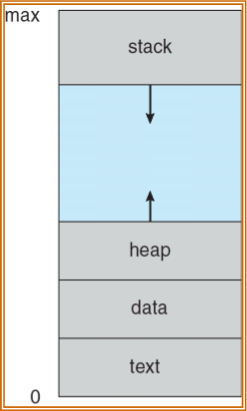
\includegraphics[scale=0.3]{images/processes_concurrency/pcb.jpg}
\caption{Process Control Block}
\end{figure}
\begin{description}
\item [Text] contains the code. This part of memory cannot be modified;
\item [Data] contains global variables;
\item [Heap] contains dynamic variables. It grows ``upward'';
\item [Stack] contains local variables and return addresses of functions. The \emph{Stack Pointer} points to the top of the stack. It grows ``downward'', i.e.,\@ in the opposite direction to the Heap.
\end{description}

It is possible to conceptually imagine the \textbf{trace} of a process as a table containing values of variables and registers (stack pointer and program counter, too) at any time, that is knowing the state of the process after any instruction. In this way it is possible to perform \emph{context switching}, the operation performed by the kernel which moves the attention of the CPU from a process to a different one, restoring its state as if it was never interrupted.

Every process has a unique identifier called \emph{PID}, a unique non negative integer. Although a PID is unique, UNIX reuses the numbers of terminated processes.

Library \texttt{unistd.h} contains system calls to retrieve PID:
\begin{verbatim}
pid_t getpid();    // Process ID
pid_t getppid();   // Parent process ID
uid_t getuid();    // Get the real user ID
gid_t geteuid();   // Get the effective ID
\end{verbatim}
\section{Concurrency}
Sequential processes are deterministic. \textit{Cooperating processes} have precedence constraints in order to guarantee a specific order in the execution. Therefore, processes are not more independent and some typical issues arise, e.g.,\@ deadlock and synchronization.

\subsection{Process creation}
System call \texttt{fork} creates a new \emph{child process} which is a perfect clone of the parent process. These processes have the same initial value of variables, they share code and file pointers of open files (pointers to the kernel memory). Instead, they do have different stacks, heaps and data sections.

\texttt{fork} returns two different values:
\begin{itemize}
\item The parent process receives the child PID: in this way it can recognize every single child;
\item The child process receives the value 0: it does not have to receive the parent PID because it can obtain it through the system call \texttt{getppid};
\item -1 in case of error.
\end{itemize}

Library \texttt{unistd.h} contains \texttt{fork} system call:
\begin{verbatim}
pid_t fork(void);
\end{verbatim}

\subsection{Process termination}
When a process terminates, the kernel sends a \texttt{SIGCHLD} to its parent. Receiving a signal is an asynchronous event and the parent process may
\begin{itemize}
\item Manage the child termination: system call \texttt{wait} and \texttt{waitpid}, or using a signal handler for signal \texttt{SIGCHLD}.
\item Ignore the event (default behavior).
\end{itemize}

System call \texttt{wait} blocks the calling process if all its children are running (none is already terminated) and it will return as soon as one of its children terminate. It returns an error if the calling process has not children.

If a parent needs to wait a specific child it is better to use \texttt{waitpid}, which suspends the execution of the calling process until the child, specified by \texttt{pid} argument, has changed state. By default \texttt{waitpid} waits only for terminated children.

Library \texttt{sys/wait.h} contains \texttt{wait} and \texttt{waitpid} system calls:
\begin{verbatim}
pid_t wait(int *statLoc);
pid_t waitpid(pid_t pid, int *statLoc, int options);
\end{verbatim}

Parameter \texttt{statLoc} is used as a return parameter which stores information about the termination of the process. There are macros to interpret its value.

\section{Move the execution}
\subsection{System call \texttt{exec}}
System call \texttt{exec} substitutes the process code with the executable code of another program. The new program begins its execution as usual from the main. In particular, the system call \texttt{exec} \textit{does not create a new process}, but it substitutes the calling process image with the image of another program and the PID does not change.

\begin{figure}[hbtp]
\centering
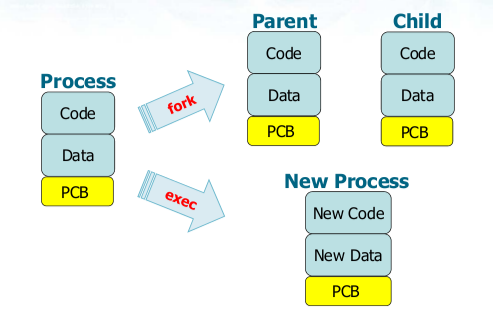
\includegraphics[scale=0.4]{images/processes_concurrency/fork_exec.png}
\caption{Different behaviors of \texttt{fork} and \texttt{exec}}
\end{figure}

There are 6 different versions of \texttt{exec} system call: \texttt{execl}, \texttt{execlp}, \texttt{execle}, \texttt{execv}, \texttt{execvp}, \texttt{execve} distinguishable by the letters:
\begin{itemize}
\item \texttt{l} (list): arguments are a list of strings. The last element must be a \texttt{NULL} pointer or equivalently, \texttt{(char *) 0};
\item \texttt{v} (vector): arguments is a vector of strings. The last element must be a \texttt{NULL} pointer or equivalently, \texttt{(char *) 0};
\item \texttt{p} (path): the executable filename is looked for in the directories listed in the environment variable \texttt{PATH};
\item \texttt{e} (environment): the last argument is an environment vector \texttt{envp[]} which defines a set of new association strings \texttt{name = value}.
\end{itemize}

Library \texttt{unistd.h} contains all the implementations of system call \texttt{exec}. They all return -1 in case of error:
\begin{verbatim}
int execl(char *path, char *arg0, ..., (char *)0);
int execlp(char *name,  char *arg0, ..., (char *)0);
int execle(char *path, char *arg0, ..., char *envp[]);
int execv(char *path, char *argv[]);
int execvp(char *name, char *argv[]);
int execve(char *path, char *argv[], char *envp[]);
\end{verbatim}

\paragraph{Arguments}
\begin{itemize}
\item Pathname of the executable file: in the `p' versions the complete path is not necessary. The file must be in one of the directories listed in the environment variable \texttt{PATH}. Remember that, for security reasons, current directory is not in \texttt{PATH};
\item Its argument list: the first argument is the \textit{name} (alias) of the process (its \texttt{argv[0]}). The other arguments of the list are arguments for the executable;
\item Possibly the environment vector.
\end{itemize}

\paragraph{UNIX shell skeleton}
\subparagraph{Command in foreground}
\begin{verbatim}
while(TRUE) {
    write_prompt;
    read_command(command, parameters);
    if(fork() == 0)
        /* Child: Execute command */
        execve(command, parameters);
    else
        /* Parent: Wait child */
        wait(&status);
}
\end{verbatim}

\subsection{System call \texttt{system}}
System call \texttt{system} forks a shell, which executes the string command, while the parent process waits the termination of the shell command.

Library \texttt{stdlib.h} contains \texttt{system} system call:
\begin{verbatim}
int system(const char *string);
\end{verbatim}

It returns:
\begin{itemize}
\item -1 or 127 in case of error;
\item The exit value of the shell that executed the command with the format of \texttt{waitpid}.
\end{itemize}

\section{Signals}
A \emph{signal} is a software interrupt\footnote{Asynchronous event which may occur at any time} sent to a process to notify it of an event that occurred. A signal can be used as a limited form of inter-process communication or for synchronization. The use of signals is prone to race conditions and they are difficult to manage.

\subsection{Generating a signal}
The UNIX command \texttt{KILL -SIGUSR1 4481} is used to send the \texttt{SIGUSR1} signal to process with PID 4481. Possible signals are \texttt{SIGUSR1}, \texttt{SIGUSR2}, \texttt{SIGALRM}, \texttt{SIGCHLD} (sent from a child process to its parent when it terminates) and \texttt{SIG\_IGN} (used to ignore a specific signal).

System call \texttt{kill} is used to send a signal \texttt{signo} to a process (or group of processes) identified by the parameter \texttt{pid}.

Library \texttt{signal.h} contains \texttt{kill} system call:
\begin{verbatim}
int kill(pid_t pid, int signo);
\end{verbatim}

\subsection{Reacting to a signal}
A process can:
\begin{itemize}
\item ignore/discard the signal. Not possible for \texttt{SIGKILL} and \texttt{SIGSTOP} which are unmaskable;
\item execute a signal handler function.
\end{itemize}
To properly react to the asynchronous arrival of a given type of signal, a process must inform the kernel about the action that it will perform when it will receive a signal of that type. Precondition to properly handle a received signal for a process is to declare to the kernel if a signal of a given type will be ignored or caught.

System call \texttt{signal} is used to inform the kernel about the reaction, specified as an address of a function \texttt{func} to execute when a specific signal \texttt{sig} is received.

Library \texttt{signal.h} contains \texttt{signal} system call:
\begin{verbatim}
void(*signal(int sig, void (*func)(int)))(int);
\end{verbatim}

The function \texttt{func} has this prototype: \texttt{void func(int signo)}. In this way, the same function can be used to manage different signals which can be recognized inside the signal handler.

\paragraph{Skeleton of a shell}
\subparagraph{Command in background (option \&)}
\begin{verbatim}
while(TRUE) {
    write_prompt;
    read_command(command, parameters);
    if(fork() == 0)
        /* Child: Execute command */
        execve(command, parameters);
    /* Parent: Continue the execution */
}
\end{verbatim}
Actually, this naive solution does not work because every child process becomes a zombie, given that there is no process waiting for it. Therefore, it is needed to allocate a signal handler which ignores the \texttt{SIGCHLD} generated on child termination: \texttt{signal(SIGCHLD, SIG\_IGN);}

\subsection{Issues}
If many signals of the \emph{same} type are waiting to be handled, then most UNIXs will only deliver one of them. So multiple signals are lost.

If many signals of \emph{different} types are waiting to be handled, they are not delivered in any fixed order.

It is good practice to re-allocate the handler at the end of the handler function. In fact, in some UNIX systems, the signal reaction is resetting to its default action immediately after the signal has been sent.

If a signal is sent during the execution of a signal handler, the signal is lost. Hence, the signal handler must be short, in order to receive
``all'' signals.

\subsection{Synchronization}
The basic idea is to allocate a signal handler and to wait the signal using the system call \texttt{pause}. When a signal is received, the process will exit from the pause and will continue its execution.

Another scenario can be obtained by using the system call \texttt{alarm}. In this way, the process informs the kernel that it wants to receive a signal (\texttt{SIGALRM}) after a given amount of time \texttt{secs}. If \texttt{secs} is set to 0, the previous alarm is canceled.
It is similar to a \texttt{sleep} but it does not block the process.

Library \texttt{unistd.h} contains both \texttt{pause} and \texttt{alarm} system calls:
\begin{verbatim}
int pause(void);
long alarm(long secs);
\end{verbatim}
\chapter{Threads}
Threads in a process share data (global variable) and code. Each threads has its own stack for function calls. Each thread can allocate its own \emph{Thread Local Storage} (TLS), which represent a way to share data which are private to the thread.

\begin{figure}[hbtp]
\centering
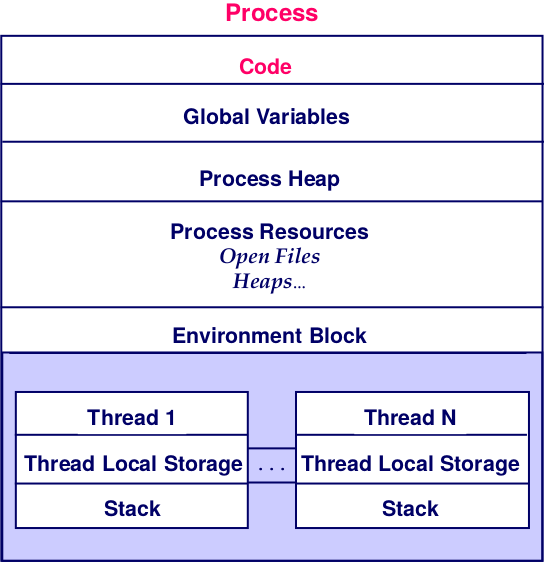
\includegraphics[scale=0.35]{images/windows_threads/process_threads.png}
\caption{Processes and threads}
\end{figure}

Threads are scheduled and run independently. Windows works with threads as atomic unit of execution and scheduling.
\\
Benefits:
\begin{itemize}
\item Simpler program models;
\item Faster code, in many cases, when it is possible to exploit multiple processors or inherent application parallelism, i.e.\@ concurrency can catch real concurrency;
\item Reliable, understandable, maintainable code.
\end{itemize}
Risks:
\begin{itemize}
\item Difficult to debug;
\item Slower performance, in some cases;
\item Potential defects.
\end{itemize}

\section{Creating a thread}
Specify the thread's start address within the process' code, specify the stack size and the stack consume space within the process' address space, 

\begin{verbatim}
HANDLE CreateThread (
  LPSECURITY_ATTRIBUTES lpsa,
  DWORD cbStack,
  LPTHREAD_START_ROUTINE lpStartAddr,
  LPVOID lpvThreadParm,
  DWORD dwCreate,
  LPDWORD lpIDThread
);
\end{verbatim}

\paragraph{Returned value}
\begin{itemize}
\item A thread's identifier value and its handle;
\item A \texttt{NULL} handle value indicates failure.
\end{itemize}

\paragraph{Parameters}
\begin{description}
\item [\texttt{lpsa}] security attributes structure, use \texttt{NULL}.
\item [\texttt{cbStack}] byte size for the new thread's stack. Use 0 to default to the primary thread's stack size (1 MB).
\item [\texttt{lpStartAddr}] points to the function to be executed. Actually it is the function name, which accepts a single pointer argument and returns a 32-bit \texttt{DWORD} exit code. The thread can interpret the argument as a \texttt{DWORD} or a pointer.
\item [\texttt{lpvThreadParm}] pointer passed as the thread argument.
\item [\texttt{dwCreate}] if zero, the thread is immediately ready to run; if \texttt{CREATE\_SUSPENDED}, the new thread will be in suspended state, requiring a \texttt{ResumeThread} function call to move the thread to the ready state.
\item [\texttt{lpIDThread}] points to a \texttt{DWORD} that receives the new thread's identifier; \texttt{NULL} is ok on W2000/NT.
\end{description}

\subsection{The thread function}
\begin{verbatim}
DWORD WINAPI MyThreadFunction(PVOID pThreadParam) {
  ExitThread (ExitCode);
  /* return ExitCode; */
}
\end{verbatim}

\section{Thread termination}
Threads are terminated by \texttt{ExitProcess}:
\begin{itemize}
\item The process and all its threads terminate;
\item The exit code returned by the thread start function is the same as the process exit code;
\end{itemize}

\begin{verbatim}
VOID ExitThread (DWORD dwExitCode);
\end{verbatim}
A thread can simply return with its exit code. \texttt{ExitThread} is preferred technique and the thread's stack is deallocated on termination. When the last thread in a process terminates, so does the process itself.

\paragraph{Parameter}
\begin{description}
\item [\texttt{dwExitCode}] the exit code for the thread.
\end{description}

It is possible to terminate a thread with \texttt{TerminateThread} but it is dangerous because the thread's stack and other resources will not be deallocated, leading to possible leaks. In fact, it is better to let the thread terminate itself.

A thread will remain in the system until the last handle to it is closed, using \texttt{CloseHandle}~\footnote{Similar to UNIX zombies}, then the thread will be deleted.

\subsection{Thread exit codes}
Any other thread can retrieve the exit code.
\begin{verbatim}
BOOL GetExitCodeThread (
  HANDLE hThread,
  LPDWORD lpdwExitCode
);
\end{verbatim}

\paragraph{Returned value}
\begin{itemize}
\item \texttt{TRUE} if the function succeeds, i.e.\@ if it is possible to retrieve the exit code;
\item \texttt{FALSE} otherwise.
\end{itemize}

\paragraph{Parameter}
\begin{description}
\item [\texttt{hThread}] handle to the thread.
\item [\texttt{lpdwExitCode}] contains the thread's exit code. It could be \texttt{STILL\_ACTIVE} if the thread is running.
\end{description}

\section{Thread identities}
A thread has a permanent \texttt{ThreadId} and it usually accessed by \texttt{HANDLE}. An \emph{ID} can be converted to a \texttt{HANDLE}.

\begin{verbatim}
HANDLE GetCurrentThread (VOID);
DWORD GetCurrentThreadId (VOID);
HANDLE OpenThread (
  DWORD dwDesiredAccess,
  BOOL InheritableHandle,
  DWORD ThreadId
);
\end{verbatim}

\paragraph{Returned value}
\begin{itemize}
\item An open \texttt{HANDLE} to the specified thread, if the function succeeds;
\item \texttt{NULL}, if it fails.
\end{itemize}

\paragraph{Parameter}
\begin{description}
\item [\texttt{dwDesiredAccess}] the access to the thread object.
\item [\texttt{InheritableHandle}] if \texttt{TRUE}, processes created by this process will inherit the handle. Otherwise, the processes do not inherit this handle.
\item [\texttt{ThreadId}] the identifier of the thread to be opened.
\end{description}

\section{Suspend \& resume threads}
Every thread has a \emph{suspend count} and it can execute only if this count is zero. A thread can be create in the \emph{suspended state} and increment or decrement the suspend count of another.

These functions are useful in preventing ``race conditions'', because they do not allow threads to start until initialization is complete but they are unsafe for general synchronization.

\begin{verbatim}
DWORD ResumeThread (HANDLE hThread);
DWORD SuspendThread (HANDLE hThread);
\end{verbatim}

\paragraph{Returned value}
\begin{itemize}
\item The previous suspend count, if the function succeeds;
\item \texttt{0xFFFFFFFF}, if it fails.
\end{itemize}

\paragraph{Parameter}
\begin{description}
\item [\texttt{hThread}] a handle to the thread to be restarted or suspended.
\end{description}

\section{Waiting for thread termination}
There is no specific function to wait for thread termination. In fact, wait for a thread to terminate using general purpose wait functions, which wait for the thread handle to become signaled.
\begin{itemize}
\item \texttt{ExitThread} and \texttt{TerminateThread} set the object to the signaled state, releasing all other threads waiting on the object;
\item \texttt{ExitProcess} sets the process' state and all it threads' states to signaled.
\end{itemize}

\begin{verbatim}
DWORD WaitForSingleObject (
  HANDLE hObject,
  DWORD dwTimeOut
);
\end{verbatim}

\paragraph{Parameters}
\begin{description}
\item [\texttt{hHandle}] a handle to the object.
\item [\texttt{dwTimeOut}] timeout interval in milliseconds.
\begin{description}
\item [\texttt{0}] means the functions returns immediately after testing the state of the specified object;
\item [\texttt{INFINITE}] for no timeout. Wait forever for a thread to terminate.
\end{description}
\end{description}

\begin{verbatim}
DWORD WaitForMultipleObjects (
  DWORD cObjects,
  LPHANDLE lphObjects,
  BOOL fWaitAll,
  DWORD dwTimeOut
);
\end{verbatim}

\paragraph{Parameters}
\begin{description}
\item [\texttt{cObjects}] is the number of handles in the array pointed to by \texttt{lphObjects}. It cannot exceed \texttt{MAXIMUM\_WAIT\_OBJECTS}, i.e.\@ 64.
\item [\texttt{lphObjects}] is an array of object handles.
\item [\texttt{fWaitAll}]
\begin{description}
\item [\texttt{TRUE}] indicates to wait for all the threads to terminate.
\end{description}
\item [\texttt{dwTimeOut}] timeout interval in milliseconds.
\begin{description}
\item [\texttt{0}] means the functions returns immediately after testing the state of the specified object;
\item [\texttt{INFINITE}] for no timeout. Wait forever for a thread to terminate.
\end{description}
\end{description}

\paragraph{Returned value}
\begin{itemize}
\item \texttt{WAIT\_OBJECT\_0}: The thread terminated, if calling \texttt{WaitForSingleObject} or \texttt{WaitForMultipleObject} with \texttt{fWaitAll} set;
\item \texttt{WAIT\_OBJECT\_0 + n}, where \texttt{0 <= n < cObjects}: Subtract \texttt{WAIT\_OBJECT} from the returned value to determine which thread terminated when calling \texttt{WaitForMultipleObject} with \texttt{fWaitAll} unset;
\item \texttt{WAIT\_TIMEOUT}: Timeout period elapsed;
\item \texttt{WAIT\_ABANDONED} Not possible with thread handles;
\item \texttt{WAIT\_FAILED}: Call \texttt{GetLastError} for thread-specific error code.
\end{itemize}

\section{The C library and threads}
Nearly all programs and thread functions use the C library, which is normally not ``thread safe'' because it uses global variables for the process, i.e.\@ for all threads and not for the single thread. The C function \texttt{\_beginthreadex} has exactly the same parameters as \texttt{CreateThread}.

Cast \texttt{\_beginthreadex} return value to \texttt{(HANDLE)} and use \texttt{\_endthreadex} in place of \texttt{ExitThread}, included in \texttt{process.h}.

\section{Synchronization objects}
A thread can wait for another to terminate (using \texttt{ExitThread} by waiting on the thread handle using \texttt{WaitForSingleObject} or \texttt{WaitForMultipleObjects}. A process can wait for another process to terminate (using \texttt{ExitProcess}) in the same way. Other common methods are reading from a pipe or socket that allows one process or thread to wait for another to write to the pipe or socket. File locks are specially for synchronizing file access.

Windows provides for other objects specifically designed for thread and process synchronization. Three are kernel objects (they have \texttt{HANDLE}s):
\begin{itemize}
\item Events, i.e.\@ specific synchronization primitive for Windows. There is no equivalence in UNIX systems;
\item Semaphores;
\item Mutexes.
\end{itemize}
Critical section is the fourth object type which can only synchronize threads within a process. Often it is the most efficient choice because it is not a kernel object and it is applicable to many scenarios. Only one thread at a time can be in a specific critical section. There is a \texttt{CRITICAL\_SECTION} type.

\subsection{\texttt{CRITICAL\_SECTION}s}
\begin{verbatim}
VOID InitializeCriticalSection (
  LPCRITICAL_SECTION lpcsCriticalSection);
VOID DeleteCriticalSection (
  LPCRITICAL_SECTION lpcsCriticalSection);
VOID EnterCriticalSection (
  LPCRITICAL_SECTION lpcsCriticalSection);
VOID LeaveCriticalSection (
  LPCRITICAL_SECTION lpcsCriticalSection);
VOID TryCriticalSection (
  LPCRITICAL_SECTION lpcsCriticalSection);
\end{verbatim}

\begin{itemize}
\item \texttt{EnterCriticalSection} blocks a thread if another thread is in the section;
\item \texttt{TryCriticalSection} simply tests if the critical section is busy, avoiding blocking;
\item \texttt{LeaveCriticalSection} unblocks waiting thread when the ``owning'' thread executes it.
\end{itemize}
Common usage is to allow threads to access global variable, which should be declared \texttt{volatile}.

\texttt{CRITICAL\_SECTION}s test in user-space, therefore they are faster because there is no kernel call. Usually they are faster than Mutexes but not always because performance is affected by different factors, e.g.\@ number of threads, number of processes and amount of thread contention.

\subsection{Mutuxes}
Mutexes can be named and have \texttt{HANDLE}s, i.e.\@ they are kernel objects. They can be used for interprocess synchronization and they are owned by a thread rather than a process.

Threads gain mutex ownership by waiting on mutex handle with standard \texttt{WaitForSingleObject} or \texttt{WaitForMultipleObjects}. Threads release ownership with \texttt{ReleaseMutex}.

A thread can acquire a specific mutex several times but must release the mutex the same number of times, e.g.\@ with nested transactions. A mutex becomes ``abandoned'' if its owning thread terminates.

\begin{verbatim}
HANDLE CreateMutex (
  LPSECURITY_ATTRIBUTES lpsa,
  BOOL fInitialOwner,
  LPCTSTR lpszMutexName
);
\end{verbatim}

\paragraph{Returned value}
\begin{itemize}
\item An open \texttt{HANDLE} to the newly created mutex object, if the function succeeds;
\item \texttt{NULL}, if it fails.
\end{itemize}

\paragraph{Parameters}
\begin{description}
\item [\texttt{lpsa}] security attributes structure, use \texttt{NULL}.
\item [\texttt{fInitialOwner}] if \texttt{TRUE}, it gives the calling thread immediate ownership of the new mutex.
\item [\texttt{lpszMutexName}] points to a null-terminated pathname. Mutexes are unnamed if it is \texttt{NULL}.
\end{description}

\begin{verbatim}
BOOL ReleaseMutex (
  HANDLE hMutex
);
\end{verbatim}
It frees a mutex that the calling thread owns and it fails if the thread does not own it.

If a mutex is abandoned, a wait will return \texttt{WAIT\_ABANDONED\_0}.

\subsubsection{Mutex naming}
Naming a mutex permits to use it in more than one process. It is not necessary to name a mutex used in a single process. Named mutex can be opened using \texttt{OpenMutex}.

\subsection{Events}
\emph{Events} can release multiple threads from a wait simultaneously when a single event in signaled, with either \texttt{PulseEvent} or \texttt{SetEvent}.

\begin{itemize}
\item A \textit{manual-reset} event can signal several threads simultaneously and must be reset by the thread;
\item A \textit{auto-reset} event signals a single thread, and the event is reset automatically.
\end{itemize}

\begin{verbatim}
HANDLE CreateEvent (
  LPSECURITY_ATTRIBUTES lspa,
  BOOL fManualReset,
  BOOL fInitialState,
  LPTCSTR lpszEventName
);
\end{verbatim}

\paragraph{Returned value}
\begin{itemize}
\item An \texttt{HANDLE} to the created event object, if the function succeeds;
\item \texttt{NULL}, if it fails.
\end{itemize}

\begin{description}
\item [\texttt{lpsa}] security attributes structure, use \texttt{NULL}.
\item [\texttt{fManualReset}] if \texttt{TRUE}, the function creates a manual-reset event object; if \texttt{FALSE}, the function creates an auto-reset event object.
\item [\texttt{fInitialState}] if \texttt{TRUE}, the initial state of the event object is signaled; otherwise, it is non-signaled.
\item [\texttt{lpszEventName}] points to a null-terminated pathname. Events are unnamed if it is \texttt{NULL}.
\end{description}
It is possible to open a named event with \texttt{OpenEvent}, possibly from another process.

\medskip
The three functions to control events are:
\begin{verbatim}
BOOL SetEvent (HANDLE hEvent);
BOOL ResetEvent (HANDLE hEvent);
BOOL PulseEvent (HANDLE hEvent);
\end{verbatim}
A thread signals an event with \texttt{SetEvent}.
\begin{itemize}
\item If the event is \textit{auto-reset}, a single waiting thread (possibly one of many) will be released and the event automatically returns to the non-signaled state. If no threads are waiting on the event, it remains in the signaled state until some thread waits on it and is immediately released.
\item If the event is \textit{manual-reset}, the event remains signaled until some thread calls \texttt{ResetEvent} for that event. During this time, all waiting threads are released. It is possible that other threads will wait, and be released, before the reset.
\end{itemize}

\texttt{PulseEvent} allows to release all threads currently waiting on a manual-reset event and the event is then automatically reset.

When using \texttt{WaitForMultipleEvents}, wait for all events to become signaled. A waiting thread will be released only when all events are simultaneously in the signaled state. Some signaled events might be released before the thread is released.

\begin{table}
\centering
\begin{tabularx}{\textwidth}{|l|X|X|}
\hline
& \multicolumn{1}{c|}{AutoReset} & \multicolumn{1}{c|}{ManualReset} \\
\hline
\texttt{SetEvent} & Exactly on e thread is released. If none are currently waiting on the event, the next thread to wait will be released. & All currently waiting threads released. The event remains signaled until reset by some thread. \\
\hline
\texttt{PulseEvent} & Exactly one thread is release, but only if a thread is currently waiting on the event. & All currently waiting threads released, and the event is then reset. \\
\hline
\end{tabularx}
\caption{Events}
\end{table}

\subsection{Semaphores}
A \emph{semaphore} combines event and mutex behavior. It can be emulated with one of each and a counter. Semaphores maintain a counter in such a way that multiple processes/threads can ``enter'' the semaphore and decrement\footnote{\texttt{P} operation} or increment\footnote{\texttt{V} operation} its counter, therefore there is no ownership.

It is possible, with care, to achieve mutual exclusion with a semaphore if it is used in binary mode and release operation is performed \emph{only when} its actually owned.

\begin{verbatim}
HANDLE CreateSemaphore (
  LPSECURITY_ATTRIBUTES lpsa,
  LONG cSemInitial,
  LONG cSemMax,
  LPCTSTR lpszSemName
);
\end{verbatim}

\paragraph{Returned value}
\begin{itemize}
\item An \texttt{HANDLE} to the semaphore object, if the function succeeds;
\item \texttt{NULL}, if it fails.
\end{itemize}

\begin{description}
\item [\texttt{lpsa}] security attributes structure, use \texttt{NULL}.
\item [\texttt{cSemInitial}] the initial count for the semaphore object. This value must be greater than or equal to zero and less than or equal to \texttt{cSemMax}.
\item [\texttt{cSemMax}] the maximum count for the semaphore object.
\item [\texttt{lpszEventName}] points to a null-terminated pathname. Events are unnamed if it is \texttt{NULL}.
\end{description}

\begin{verbatim}
BOOL ReleaseSemaphore (
  HANDLE hSemaphore,
  LONG cReleaseCount,
  LPLONG lpPreviousCount
);
\end{verbatim}

\paragraph{Returned value}
\begin{itemize}
\item An \texttt{TRUE}, if the function succeeds;
\item \texttt{FALSE}, if it fails.
\end{itemize}

\begin{description}
\item [\texttt{hSemaphore}] handle to the semaphore object.
\item [\texttt{cReleaseCount}] the amount by which the counter is to be increased. The value must be greater than zero. If the specified amount would cause the counter to exceed the maximum count, the count is not changed and the function returns FALSE.
\item [\texttt{lpPreviousCount}] a pointer to a variable to receive the previous count for the semaphore. This parameter can be \texttt{NULL} if the previous count is not required.
\end{description}
\chapter{Synchronization}
In concurrent programming where processes or threads cooperate and share data, race conditions may arise and there may be sections of not-reentrant code, it is needed to properly synchronize the cooperating actors to make their results not dependent on their relative speed.

A \emph{Critical Section} or \emph{Critical Region} is a section of code, common to multiple threads, in which they can access shared objects or in which they are competing for the use of shared resources. It is needed to ensure that when one thread is executing in its critical section, no other thread is allowed to execute in its critical section, therefore an access protocol must be established to enter the critical section in \textbf{mutual exclusion}:

\begin{itemize}
\item A thread executes a ``reservation'' code before entering a CS;
\item The reservation code blocks the thread if another is using its CS;
\item Leaving its CS, a thread executes a code to release the CS;
\item The release possibly unlocks another thread which was waiting in the ``reservation'' code of its CS.
\end{itemize}

In general, the \textbf{software solutions} to the problem of CS are complex and inefficient. In fact, test and set operations are ``invisible'' to the other threads and they are not atomic, thus a thread can react to the presumed value of a variable rather than to its current value. Furthermore, the solutions is not easily extensible to an arbitrary number of threads.

The \textbf{hardware solutions} can be easily extensible to a larger number of threads but they introduce busy form of waiting with spin lock leading to possible starvation.

\section{Semaphores}
The hardware solution can be used to implement system calls that can be used for solving every kind of synchronization problem (not only the Mutual Exclusion) avoiding the busy form of waiting. These system calls rely on a data structure introduce by Dijkstra in 1965 called semaphore.

A \emph{semaphore} is a shared structure including a counter, a waiting queue managed by the kernel both protected by a lock.
The kernel offers a set of \textbf{atomic primitives} that allows a thread to be blocked on the semaphore or to wake up if it was locked.

\begin{description}
\item \texttt{init(S, k)} defines and initializes semaphore \texttt{S} counter to value \texttt{k}. \texttt{k} is a positive value because the system calls manage the counter so that, if negative, its absolute value is the number of threads waiting on the semaphore queue.
\item \texttt{wait(S)} decrements the counter and blocks the calling thread if the counter value of \texttt{S} is negative or zero.
\item \texttt{signal(S)} increases the counter and made some blocked threads ready to run if the counter value of \texttt{S} is negative or zero.
\item \texttt{destroy(S)} releases semaphore \texttt{S} memory.
\end{description}

Semaphores can be used to solve any synchronization problem using an appropriate protocol, possibly adding more than one semaphore and additional share variables.

\subsection{POSIX semaphores}
POSIX semaphores define a set of kernel independent system calls, included in header file \texttt{semaphore.h} which return -1 on error.

\begin{description}
\item \texttt{int sem\_init(sem\_t *sem, int pshared, usigned int value)} initializes the semaphore counter at value \texttt{value}. The \texttt{pshared} value identifies the type of semaphore. If it is equal to 0, the semaphore is local to the threads of current process, otherwise the semaphore can be shared between different processes.

\item \texttt{int sem\_wait(sem\_t *sem)} implements the standard wait, i.e.\@ if the counter is negative or zero, the calling thread is blocked.

\item \texttt{int sem\_post(sem\_t *sem)} implements the standard signal, i.e.\@ increments the counter and wakes up a blocking thread if the counter is negative or zero.

\item \texttt{int sem\_getvalue(sem\_t *sem, int *valP)} allows obtaining the value of the semaphore counter. The value is assigned to \texttt{*valP}.

\item \texttt{int sem\_destroy(sem\_t *sem)} destroys the semaphore at the address pointed by \texttt{sem}.

\item \texttt{int sem\_trywait(sem\_t *sem)} implements a non-blocking wait, i.e.\@ if the semaphore counter has a value greater than 0, it performs the decrement and returns 0 while, if the semaphore counter is negative or zero, it returns -1 instead of blocking the caller as \texttt{sem\_wait} does.
\end{description}

\subsection{Pthread mutex}
Pthread mutex defines binary semaphores of type \texttt{pthread\_mutex\_t} by means of system calls
\begin{description}
\item \texttt{int pthread\_mutex\_init(pthread\_mutex\_t *mutex, \newline const pthread\_mutexattr\_t *attr)} initializes the mutex referenced by \texttt{mutex} with attributes specified by \texttt{attr} (default = \texttt{NULL}).

\item \texttt{int pthread\_mutex\_lock(pthread\_mutex\_t *mutex)} blocks the caller if the \texttt{mutex} is locked or acquires the mutex lock if the \texttt{mutex} is unlocked.

\item \texttt{int pthread\_mutex\_trylock(pthread\_mutex\_t *mutex)} is similar to a \texttt{lock}, but returns without blocking the caller if \texttt{mutex} is locked. It returns 0 if the lock has been successfully acquired or a \texttt{EBUSY} error if  the \texttt{mutex} was already locked.

\item \texttt{int pthread\_mutex\_unlock(pthread\_mutex\_t *mutex)} releases the \texttt{mutex} lock.

\item \texttt{int pthread\_mutex\_destroy(pthread\_mutex\_t *mutex)} frees \texttt{mutex} memory so that it cannot be used anymore.
\end{description}

\section{Synchronization protocols with semaphores}
\subsection{Producer \& Consumer with limited memory buffer}
This problem uses a circular buffer implementing a FIFO queue of size \texttt{MAX} for storing the produced elements to be consumed. If the buffer is empty, the consumer has to wait. On the other hand, if the buffer is full, the producer has to wait. In an intermediate situation, producer and consumer can produce and consume in a concurrent fashion.

\begin{figure}[hbtp]
\centering
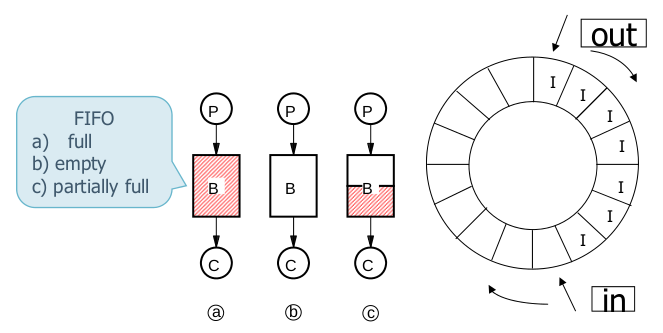
\includegraphics[scale=0.4]{images/synchronization/producer_consumer_buffer.png}
\caption{Circular buffer}
\end{figure}

\paragraph{Access functions}
Functions without considering synchronization and concurrency.
\begin{Parallel}{}{}
\ParallelLText{
\begin{verbatim}
void enqueue(int val) {
  queue[in] = val;
  in = (in + 1) % MAX;
  return;
}
\end{verbatim}}
\ParallelRText{
\begin{verbatim}
void dequeue(int *val) {
  queue[out] = val;
  out = (out + 1) % MAX;
  return;
}
\end{verbatim}}
\end{Parallel}

\paragraph{Concurrent access}
Initially, a consumer has to wait and a producer has to produce, i.e.\@ it has not to be blocked. Therefore, a consumer has to wait on full, initialized to 0 and a producer has to produce at most \texttt{MAX} elements. Both signal when an elements is enqueued or dequeued.
\begin{verbatim}
init(full, 0);
init(empty, MAX);
\end{verbatim}

\begin{Parallel}{}{}
\ParallelLText{
\begin{verbatim}
Producer() {
  Message m;
  while(TRUE) {
    produce(m);
    wait(empty);
    enqueue(m);
    signal(full);
  }
}
\end{verbatim}}
\ParallelRText{
\begin{verbatim}
Consumer() {
  Message m;
  while(TRUE) {
    wait(full);
    m = dequeue();
    signal(empty);
    consume(m);
  }
}
\end{verbatim}}
\end{Parallel}

Producer and consumer operate on different indexes of the buffer, thus they can operate in concurrency as long as the queue is not full or empty, otherwise either a producer or a consumer is blocked.

The solution is symmetric and it can be easily extended to more than one producer and consumer processes, remembering that operations on the queue are not atomic and multiple consumers or multiple producers must act in mutual exclusion.

\paragraph{Producers \& Consumers}
\begin{verbatim}
init(full, 0);
init(empty, MAX);
init(meP, 1);
init(meC, 1);
\end{verbatim}

\begin{Parallel}{}{}
\ParallelLText{
\begin{verbatim}
Producer() {
  Message m;
  while(TRUE) {
    produce(m);
    wait(empty);
    wait(meP);
    enqueue(m);
    signal(meP);
    signal(full);
  }
}
\end{verbatim}}
\ParallelRText{
\begin{verbatim}
Consumer() {
  Message m;
  while(TRUE) {
    wait(full);
    wait(meC);
    m = dequeue();
    signal(meC);
    signal(empty);
    consume(m);
  }
}
\end{verbatim}}
\end{Parallel}

\newpage

\subsection{Readers \& Writers}
This represents the typical problem of sharing a database between two sets of concurrent threads:
\begin{itemize}
\item Readers are allowed to access the database in concurrency;
\item Writers must access the database in Mutual Exclusion with other Writers and Readers.
\end{itemize}
When a writer is writing in the database, several Readers and Writers processes can be blocked waiting the end of the write operation.

\textbf{Readers precedence}: at the end of a writing operation, favour the access of the waiting Readers rather than of the waiting Writers.

\textbf{Writers precedence}: at the end of a writing operation, favour the access of the waiting Writers rather than of the waiting Readers.

\paragraph{Readers priority}
Giving priority to the Readers means that a Reader does not wait unless a Writer is writing.

While Readers are reading, new Readers are allowed to read and Writers are blocked. The first Reader blocks any Writer and, dually, when the last Reader terminates, a waiting Writer can access the database.

The solution uses:
\begin{itemize}
\item A shared variable \texttt{nR} that counts the number of Readers inside the critical section;
\item A Mutual Exclusion semaphore \texttt{meR} to protect variable \texttt{nR};
\item A Mutual Exclusion semaphore \texttt{w} among Writers or among Readers and Writers;
\item A Mutual Exclusion semaphore \texttt{meW} among Writers.
\end{itemize}

\begin{verbatim}
nR = 0;
init(meR, 1);
init(meW, 1);
init(w, 1);
\end{verbatim}

\begin{Parallel}{}{}
\ParallelLText{
\begin{verbatim}
Reader() {
  wait(meR);
    nR++;
    if(nR == 1)
      wait(w);
  signal(meR);
  // read
  wait(meR);
    nR--;
    if(nR == 0)
      signal(w);
  signal(meR);
}
\end{verbatim}}
\ParallelRText{
\begin{verbatim}
Writer() {
  wait(meW);
  wait(w);
  // write
  signal(w);
  signal(meW);
}
\end{verbatim}}
\end{Parallel}

\paragraph{Writers priority}
Giving priority to the Writers means that a Writer has priority over all Readers.

A Writer trying to enter its critical section blocks \emph{new} Readers, but the Readers that are inside their critical section are allowed to complete their reading task.

The solution uses:
\begin{itemize}
\item Two shared variables \texttt{nR} and \texttt{nW} to count the Readers inside the critical section and the Writers that need to write (one of them possibly writing);
\item Two Mutual Exclusion semaphores \texttt{meR} and \texttt{meW} to protect the variables \texttt{nR} and \texttt{nW};
\item Two Mutual Exclusion semaphores \texttt{r} and \texttt{w} to enforce Readers and Writers to wait on different queues.
\end{itemize}

\begin{verbatim}
nR = nW = 0;
init(meR, 1);
init(meW, 1);
init(w, 1);
init(r, 1);
\end{verbatim}

\begin{Parallel}{}{}
\ParallelLText{
\begin{verbatim}
Reader() {
  wait(r);
    wait(meR);
      nR++;
      if(nR == 1)
        wait(w);
    signal(meR);
  signal(r);
  // read
  wait(meR);
    nR--;
    if(nR == 0)
      signal(w);
  signal(meR);
}
\end{verbatim}}
\ParallelRText{
\begin{verbatim}
Writer() {
  wait(meW);
    nW++;
    if(nW == 1)
      wait(r);
  signal(meW);
  wait(w);
  // write
  signal(w);
  wait(meW);
    nW--;
    if(nW == 0)
      signal(r);
  signal(meW);
}
\end{verbatim}}
\end{Parallel}

\subsection{Single lane tunnel}
A tunnel has a single lane, and cars can proceed only in alternate directions. Therefore it is needed to enable any number of cars (threads) to proceed in the same direction and block traffic in one direction if there is traffic in the opposite one.

\begin{figure}[hbtp]
\centering
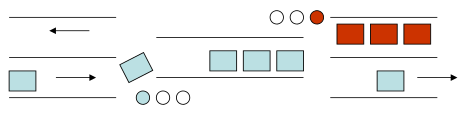
\includegraphics[scale=0.4]{images/synchronization/single_lane_tunnel.png}
\caption{Single lane tunnel}
\end{figure}


This problem is similar the Readers \& Writers one, but for two sets of Readers. In its basic implementation can result in starvation of cars in one direction.

The solution uses:
\begin{itemize}
\item Two shared count variables \texttt{n1} and \texttt{n2}, one for each travel direction;
\item Two semaphores \texttt{s1} and \texttt{s2}, one for each travel direction;
\item A global semaphore wait \texttt{busy}.
\end{itemize}

\begin{verbatim}
n1 = n2 = 0;
init(s1, 1);
init(s2, 1);
init(busy, 1);
\end{verbatim}

\begin{Parallel}{}{}
\ParallelLText{
\begin{verbatim}
left2right() {
  wait(s1);
    n1++;
    if(n1 == 1)
      wait(busy);
  signal(s1);
  // run left to right
  wait(s1);
    n1--;
    if(n1 == 0)
      signal(busy);
  signal(s1);
}
\end{verbatim}}
\ParallelRText{
\begin{verbatim}
right2left() {
  wait(s2);
    n2++;
    if(n2 == 1)
      wait(busy);
  signal(s2);
  // run right to left
  wait(s2);
    n2--;
    if(n" == 0)
      signal(busy);
  signal(s2);
}
\end{verbatim}}
\end{Parallel}

\subsection{Conditions}
A \emph{condition} is a data structure containing a mutual exclusion lock, a condition variable and a data structure to protect because it require synchronization.

\begin{verbatim}
typedef struct Cond {
  pthread_mutex_t lock;
  pthread_cond_t mycond;
  int i;
} Cond;
\end{verbatim}

\begin{description}
\item \texttt{lock} protects the structure;
\item \texttt{mycond} is the condition variable;
\item \texttt{i} is the variable to set or check.
\end{description}

Main thread has to define such a structure, allocate a global structure of that type, initialize its variables and create two threads A and B.

Thread A does work until it needs to check a given condition by calling \texttt{pthread\_cond\_wait} to wait for a signal from thread B, unlocking the lock (otherwise, no one can change the variable content). When signaled, thread A wakes up with lock locked and, after explicitly unlocking the lock, can continues its work.

Thread B does work and locks the condition lock. It changes the value of the global variable associated to the waiting condition and, if thread A wait condition is true, it performs a \texttt{pthread\_cond\_signal}. After unlocking the condition lock, it can continue its work.

\paragraph{Waiting on Condition Variables}
\begin{description}
\item \texttt{int pthread\_cond\_wait(pthread\_cond\_t *cond, \newline pthread\_mutex\_t *mutex)} blocks the calling thread until the specified condition is signaled. This system call should be called while \textit{lock} is locked, and it will automatically release the \textit{lock} while it waits.

After signal is received and thread is awakened, lock be automatically locked for use by the thread.

The programmer is then responsible for unlocking lock when the thread does not more need it.
\end{description}

\paragraph{Signaling on Condition Variables}
\begin{description}
\item \texttt{int pthread\_cond\_signal(pthread\_cond\_t *cond)} signals another thread which is waiting on the condition variable.

It should be called with the \textit{lock} locked, and must unlock the \textit{lock} to allow \texttt{pthread\_cond\_wait} to complete.

\item \texttt{int pthread\_cond\_broadcast(pthread\_cond\_t *cond)} \newline
should be used if more than one thread is blocked on the same condition variable, rather than \texttt{pthread\_cond\_signal}. It is a logical error to call \texttt{pthread\_cond\_signal} before calling \texttt{pthread\_cond\_wait}.
\end{description}

\subsection{Precedence graphs}
Goal is to implement a graph using the minimum number of semaphores remembering that signals are sent to a semaphore, not to a process and they are caught by the first process able to receive them.

The first thing to do is to delete arcs which are not necessary and can, therefore, lead to use a non minimum number of semaphores.

\textbf{Acyclic threads}: outgoing arcs require a single semaphore and incoming arcs require a single semaphore.

\textbf{Cyclic threads}: outgoing arcs require different semaphores, while incoming arcs use a single  semaphore. In fact, using the same semaphore, because of the loop statement, a single process can get two signals if it is very fast.
\chapter{Memory management}
Memory is an important module in the operating system because without it, it is impossible to run a program. In a multi-user or multi-programming environment, CPU needs to share memory and kernel must manage it offering the concept of \emph{virtual memory} to the processes, by using external devices and differentiating between real and virtual memory (swapping partition).

A pair of \textbf{base} and \textbf{limit} registers defines the logical address space and via hardware it is checked that the process remains in its space.

\begin{figure}[hbtp]
\centering
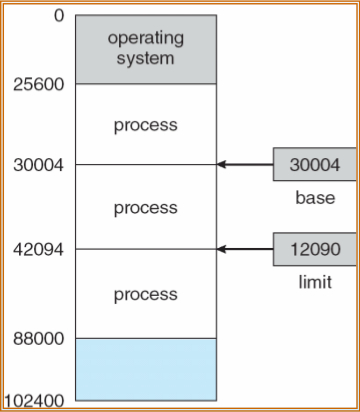
\includegraphics[scale=0.4]{images/memory_management/base_limit_regs.jpg}
\caption{Base and limit registers}
\end{figure}

Address biding of instructions and data to memory addresses can happen at three different stages:

\begin{itemize}
\item \textbf{Compile time}: If memory location is known a priori, \emph{absolute code} can be generated which must be recompiled if starting location changes;
\item \textbf{Load time}: If memory location is not known at compile time, \emph{relocatable code} must be generate;
\item \textbf{Execution time}: If the process can be moved during its execution from one memory to another, binding is delayed until run time and hardware support is needed for address mapping.
\end{itemize}

\begin{figure}[hbtp]
\centering
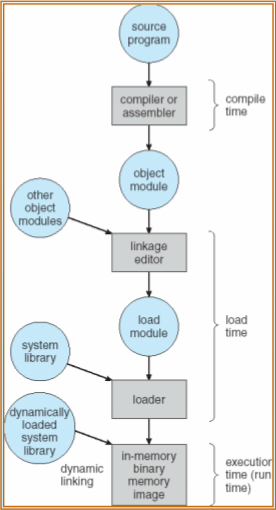
\includegraphics[scale=0.4]{images/memory_management/multistep_processing.jpg}
\caption{Multistep processing}
\end{figure}

Old CPUs generated ``static'' programs with pre-defined space and starting address, while modern CPUs generate logical address, starting from 0, mapped by the loader and the kernel into a physical one. In fact, loader interacts with the kernel, knowing which part of the memory are free and where to locate the program.
Addresses are always logical contiguous but pages are located around the memory, therefore the design is more complicated but more flexible, too.

\begin{itemize}
\item \textbf{Logical addresses} or \textbf{virtual addresses} are generated by the CPU;
\item \textbf{Physical addresses} are the addresses seen by the memory unit.
\end{itemize}
Logical and physical addresses are the same in compile time and load time address binding schemes; logical and physical addresses differ in execution time address binding scheme.

\subsection*{Memory management unit}
\emph{Memory management Unit} is the hardware device responsible of mapping a virtual address into a physical one. The value in the \emph{relocation register} is added to every address generated by a user process at the time it is sent to memory. User programs deal with logical address, never with real physical addresses.

\begin{figure}[hbtp]
\centering
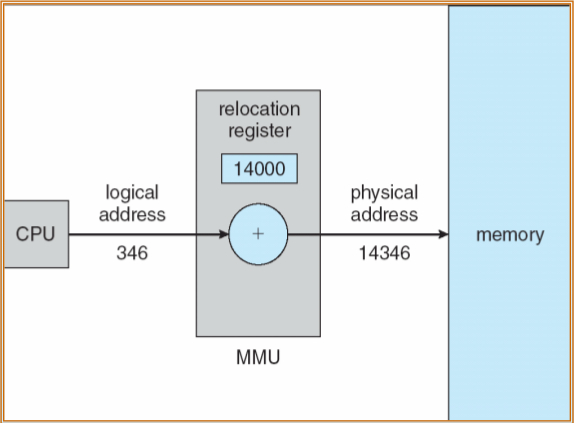
\includegraphics[scale=0.35]{images/memory_management/relocation_register.jpg}
\caption{Relocation register. From logical to physical address}
\end{figure}

\textbf{Dynamic loading} permits to load a routine on need. It is useful when large amounts of code are needed to handle infrequently occurring cases. In fact, an unused routine is never loaded, leading to a better memory-space utilization. No special support from the operating system is required, because it is implemented through program design.

\textbf{Dynamic linking} permits to postpone linking until execution time. A small piece of code, \emph{stub}, is used to locate the appropriate memory-resident library routine. Stub replaces itself with the address of the routine and executes the routine. Operating system needs to check if the routine is in processes' memory address. It is particularly useful for libraries.

\paragraph{Swapping}
A process can be temporarily swapped out of memory to a backing store and then brought back into memory to continue its execution. \emph{Backing store} is a fast disk large enough to accommodate copies of all memory images for all users, which must provide direct access to these memory images. The system maintains a \textbf{ready queue} of ready-to-run processes which have memory images on disk. \emph{Roll out, roll in} is a swapping variant used for priority-based scheduling algorithms: lower-priority process is swapped out so higher-priority process can be loaded and executed.

Major part of swap time is transfer time and the total transfer time is directly proportional to the amount of swapped memory.

\section{Contiguous allocation}
Usually, main memory is divided into two partitions:

\begin{itemize}
\item Resident operating system, usually held in low memory with interrupt vector;
\item User processes held in high memory.
\end{itemize}
Relocation registers are used to protect user processes from each other, and from changing operating system code and data. Memory management unit dynamically maps logical addresses.

When a process arrives, it is allocated memory from a hole\footnote{Block of available memory. Holes of various size are scattered throughout memory.} large enough to accommodate it. Operating system maintains information about allocated partitions and free partitions (holes). Different algorithms are available to satisfy a request from a list of free holes.

\begin{itemize}
\item \textbf{First-fit} allocates the first hole that is big enough;
\item \textbf{Best-fit} allocates the smallest hole that is big enough; it must scan the entire list, unless it is ordered by size, and produces the smallest leftover hole;
\item \textbf{Worst-fit} allocates the largest hole; it must scan the entire list too and produces the largest leftover hole.
\end{itemize}
First-fit and best-fit are better than worst-fit in terms of speed and storage utilization.

\paragraph{Fragmentation}
\begin{itemize}
\item \textbf{External Fragmentation}: total memory space exists to satisfy a request, but it is not contiguous;
\item \textbf{Internal Fragmentation}: allocated memory may be slightly larger than requested memory; this size difference is memory internal to a partition but not being used.
\end{itemize}
External fragmentation can be reduced by \emph{compaction} which is possible only if relocation is dynamic, it is done at execution time and implies to shuffle memory contents to place all free memory together in one large block.

\section{Paging}
Physical memory is divided into fixed-size blocks called \textbf{frames} and logical memory is divided into blocks of the same size called \textbf{pages}. In this way, logical address space of a process can be \emph{non-contiguous} and a process can be allocated in physical memory whenever the latter is available.

Each address generated by the CPU is divided into:
\begin{itemize}
\item \textbf{Page number}: used as an index into a \emph{page table} which contains base address of each page in physical memory;
\item \textbf{Page offset}: combined with base address to define the physical memory address that is sent to the memory unit.
\end{itemize}

\paragraph{Page table} \emph{Page table} is kept in main memory, identified by \textbf{Page table base register (PTBR)} pointing to the page table and \textbf{Page table length register (PRLR)} indicating size of the page table.

In this scheme, every access requires two memory accesses, the first one for the page table and the second one for the data/instruction. The two memory access problem can be solved by means of a special fast-lookup hardware cache called \emph{associative memory} or \textbf{translation look-aside buffer (TLB)}. An associative memory provides an address given a content, i.e.\@ the opposite behavior with respect to a canonical memory.

\begin{figure}[hbtp]
\centering
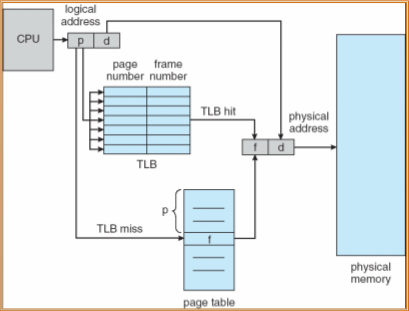
\includegraphics[scale=0.5]{images/memory_management/address_generation_tlb.jpg}
\caption{Address generation with TLB}
\end{figure}

Being $\epsilon$ the time for associative lookup, $t$  the cycle time and $\alpha$ the hit ratio, the \textbf{Effective Access Time} is calculated as $\text{EAT} = (t + \epsilon) \alpha + (2 t + \epsilon)(1 - \alpha)$

\paragraph{Memory protection} Memory protection is implemented by associating a protection bit with each frame. A \emph{valid-invalid bit} is attached to each entry in the page table:

\begin{itemize}
\item \textbf{Valid} indicates that the associated page is in the process' logical address space, and is therefore a legal page;
\item \textbf{Invalid} indicates that the page is not in the process' logical address space.
\end{itemize}
TLB is an hardware structure and therefore shared. Hence, it has to be rebuilt on context switch.

One copy of read-only code can be shared among processes (i.e.\@ text editors, compilers, window systems). Shared code must appear in the same location in the logical address space of all processes.

On the other hand, each process keeps a separate copy of the code and data. Pages for the private code and data can appear anywhere in the logical address space. Page table is inherited by a child process, in fact parent and child processes execute the same code and share the initial status. A new frame will be allocated by the process if it changes some variable content.

\subsection{Structure of the page table}
Having $n$ bits to store the page number, in kernel memory it is needed to have $2^n$ entries to store the page table.
\paragraph{Hierarchical Page Table} \emph{Hierarchical Page Table} breaks up the logical address space into multiple page tables. A simple technique is a two-level page table.

For example, a logical address on 32-bit machine with 1K page size is divided into:
\begin{itemize}
\item a page number consisting of 22 bits;
\item a page offset consisting of 10 bits.
\end{itemize}
Since the page table is paged, the page number is further divided into
\begin{itemize}
\item a 12-bit page number;
\item a 10-bit page offset.
\end{itemize}

\begin{figure}[hbtp]
\centering
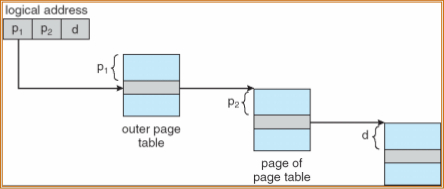
\includegraphics[scale=0.4]{images/memory_management/two_levels_pagetable.jpg}
\caption{Two levels page table}
\end{figure}

\paragraph{Hashed Page Table}
\emph{Hashed Page Table} is common in address space larger than 32 bits. The virtual page number is hashed into a page table containing a chain of elements hashing to the same location. Virtual page numbers are compared in this chain searching for a match and, if a match is found, the corresponding physical frame is extracted.

\begin{figure}[hbtp]
\centering
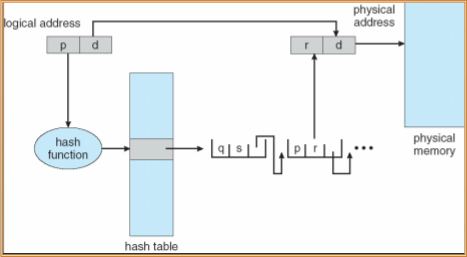
\includegraphics[scale=0.4]{images/memory_management/hashed_pagetable.jpg}
\caption{Hashed page table}
\end{figure}

\paragraph{Inverted Page Table}
\emph{Inverted Page Table} contains one entry for each real page memory. Each entry consists of the virtual address of the page stored in the real memory location, with information about the process which owns that page. This solution decreases the amount of needed memory to store each page table, but increases time needed to search the table when a page reference occurs.

\begin{figure}[hbtp]
\centering
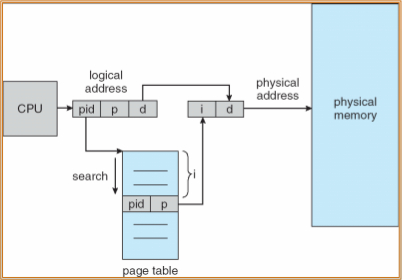
\includegraphics[scale=0.4]{images/memory_management/inverted_pagetable.jpg}
\caption{Inverted page table}
\end{figure}

\section{Segmentation}
\emph{Segmentation} is a memory management scheme which supports user view of memory. In fact, a program is a collection of segments\footnote{A segment is a logical unit containing homogeneous data with a variable size.}. Logically, an address consists of a two tuple composed by segment number and offset.

Segment table is identified by a \textbf{Segment table base register (STBR)}  pointing to the segment table's location in memory and \textbf{Segment table length register (STLR)} indicating the number of segments used by a program. Segment table maps two-dimensional physical addresses; each table entry has
\begin{itemize}
\item \textbf{Base}: contains the starting physical address where the segment resides in memory;
\item \textbf{Limit}: specifies the length of the segment.
\end{itemize}

Protection is ensured associating a validation bit and read/write/execute privileges to each entry in segment table. Since segments vary in length, memory allocation is a dynamic storage allocation problem.

\section*{Memory mapping}
Instruction \texttt{mmap} allocates some memory for a file. It is useful if the file has to be read in a non-sequential way. In this way, file is seen as a memory array and the programmer does not care about reading or moving on the file because it is transparently done by the kernel.
Library \texttt{sys/mman.h} contains \texttt{mmap} function:
\newline
\texttt{void *mmap(void *addr, size\_t len, int prot, int flags, \\ int fd, off\_t off)}

It maps \texttt{len} bytes starting at offset \texttt{off} from the file specified by the file descriptor \texttt{fd} into the caller's address space and it returns the actual place where the object is mapped. \texttt{addr} is a hint only where to allocate the file, and is usually specified as 0 (\texttt{NULL}).

\texttt{prot} describes the desired memory protection as the bitwise or of \texttt{PROT\_READ}, \texttt{PROT\_WRITE} and \texttt{PROT\_EXEC}.

\texttt{FLAGS} is the bitwise or of
\begin{itemize}
\item \texttt{MAP\_SHARED}: any update made to the mapped region will be global, i..e\@ it will be seen by any other process (common option);
\item \texttt{MAP\_PRIVATE}: updates will be kept private to each process, copy on write;
\item Many other options on Linux.
\end{itemize}
\chapter{Virtual memory}
\emph{Virtual memory} provides a separation of user logical memory from physical memory. Only part of the program needs to be in memory for execution, therefore logical address space can be much larger than physical address space. Virtual memory allows address spaces to be shared by several processes and it allows a more efficient process creation. It can be implemented via demand paging or demand segmentation.

\section{Demand paging}
\emph{Demand paging} consists of bringing a page into memory only when it is needed, leading to less input/output operations, less memory needed and faster response. An invalid reference causes an abort, while a not-in-memory fault causes a page fault exception.

Demand paging works because of the locality model. In fact, process migrates from one locality to another. These localities may overlap.

With each entry in the page table, a valid-invalid bit is associated, initially set to invalid (i.e.,\@ not-in memory) on all entries. During address translation, if valid-invalid bit in page table entry is set to invalid, a page fault occurs.

A swapper that deals with pages is a \textbf{pager}.

\paragraph{Page fault}
If there is a reference to a page, first reference to that page will trap the operating system: \emph{page fault}.
\begin{enumerate}
\item Operating system looks at another table to decide:
\begin{itemize}
\item Invalid reference $\Rightarrow$ abort;
\item Just not in memory;
\end{itemize}
\item Get empty frame;
\item Swap page into frame;
\item Reset tables;
\item Set validation bit;
\item Restart the instruction that caused the page fault.
\end{enumerate}

\begin{figure}[hbtp]
\centering
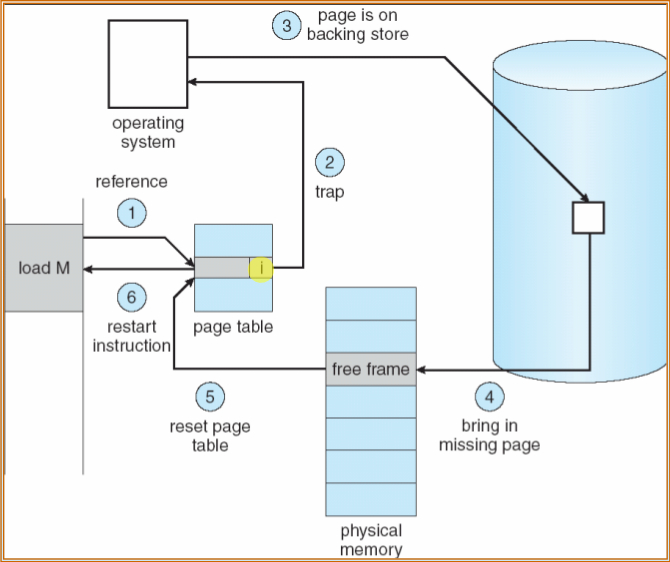
\includegraphics[scale=0.4]{images/virtual_memory/page_fault.jpg}
\caption{Page fault handling}
\end{figure}

$\text{EAT} = (1-p) t_{\text{memory}} + p (t_{\text{page fault}} + t_{\text{swap out}} + t_{\text{swap in}} + t_{\text{restart}})$ being $ 0 \le p \le 1 $, page fault ratio.

\subsection{Page replacement}
If there is no free frame, it is needed to find some page in memory not really in use and swap it out.
\begin{itemize}
\item Prevent over-allocation of memory by modifying page-fault service routine to include page replacement;
\item Use modify (dirty) bit to reduce overhead of page transfers: only modified pages are written to disk;
\item Page replacement completes separation between logical and physical memory. Larger virtual memory can be provided on a smaller physical memory.
\end{itemize}

\paragraph{Basic algorithm}
\begin{enumerate}
\item Find the location of the desired page on disk;
\item Find a free frame:
\begin{itemize}
\item If there is a free frame, use it;
\item If there is no free frame, use a page replacement algorithm to select a victim frame;
\end{itemize}
\item Bring the desired page into the newly free frame and update page and frame tables;
\item Restart the process.
\end{enumerate}

\paragraph{Optimal Algorithm}
Replace page that will not be used for longest period of time. Used for measuring every algorithm performance. It is unfeasible because it should predict the future.

\paragraph{FIFO Algorithm}
\begin{center}
\begin{tabular}{l|cccccccccccc}
\hline
Time & 1 & 2 & 3 & 4 & 5 & 6 & 7 & 8 & 9 & 10 & 11 & 12 \\
\hline
String & 4 & 3 & 2 & 1 & 4 & 3 & 5 & 4 & 3 & 2 & 1 & 5 \\
\hline
Fault & • & • & • & • & • & • & • &  &  & • & • &  \\
\hline
Frame 1 & 4 & 3 & 2 & 1 & 4 & 3 & 5 & 5 & 5 & 2 & 1 & 1 \\
Frame 2 & & 4 & 3 & 2 & 1 & 4 & 3 & 3 & 3 & 5 & 2 & 2 \\
Frame 3 &  &  & \textbf{4} & \textbf{3} & \textbf{2} & \textbf{1} & 4 & 4 & \textbf{4} & \textbf{3} & 5 & 5 \\
\hline
\end{tabular}
\[ f = 9/12 = 75 \% \]
\end{center}
This algorithm is subjected to Belady's Anomaly: adding more frames will cause more page faults.

\begin{figure}[hbtp]
\centering
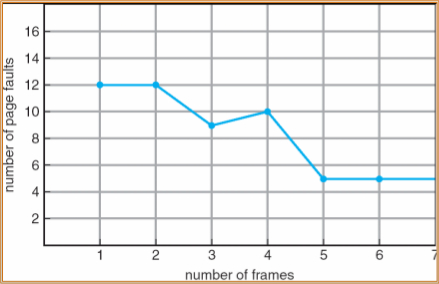
\includegraphics[scale=0.4]{images/virtual_memory/belady_anomaly.jpg}
\caption{Belady's Anomaly}
\end{figure}

\paragraph{Least Recently Used Algorithm}
Every page entry has a counter; every time page is referenced through this entry, the clock is copied into the counter. When a page needs to be changed, look at the counters to determine which are to change.

\begin{center}
\begin{tabular}{l|cccccccccccc}
\hline
Time & 1 & 2 & 3 & 4 & 5 & 6 & 7 & 8 & 9 & 10 & 11 & 12 \\
\hline
String & 4 & 3 & 2 & 1 & 4 & 3 & 5 & 4 & 3 & 2 & 1 & 5 \\
\hline
Fault & • & • & • & • & • & • & • & & & • & • & • \\
\hline
Frame 1 & 4 & 3 & 2 & 1 & 4 & 3 & 5 & 4 & 3 & 2 & 1 & 5 \\
Frame 2 & & 4 & 3 & 2 & 1 & 4 & 3 & 5 & 4 & 3 & 2 & 1 \\
Frame 3 & & & \textbf{4} & \textbf{3} & \textbf{2} & \textbf{1} & 4 & 3 & \textbf{5} & \textbf{4} & \textbf{3} & 2 \\
\hline
\end{tabular}
\[ f = 10/12 = 83 \% \]
\end{center}

A possible implementation is the \textbf{stack implementation} which keeps a stack of page numbers in a double link form:
\begin{itemize}
\item Page referenced
\begin{itemize}
\item Move it to the top;
\item Requires six pointers to be changed;
\end{itemize}
\item No search for replacement.
\end{itemize}
This implementation causes a large overhead and therefore is unfeasible and not used in reality.

\subparagraph{Least Recently Used Stack}
Adding a new page cannot increase the number of page faults. In fact, the old ``stack'' is the same and it can keep a new page.
\begin{center}
\begin{tabular}{l|cccccccccccc}
\hline
Time & 1 & 2 & 3 & 4 & 5 & 6 & 7 & 8 & 9 & 10 & 11 & 12 \\
\hline
String & 4 & 3 & 2 & 1 & 4 & 3 & 5 & 4 & 3 & 2 & 1 & 5 \\
\hline
Fault & • & • & • & • & & & • & & & • & • & • \\
\hline
Frame 1 & 4 & 3 & 2 & 1 & 4 & 3 & 5 & 4 & 3 & 2 & 1 & 5 \\
Frame 2 & & 4 & 3 & 2 & 1 & 4 & 3 & 5 & 4 & 3 & 2 & 1 \\
Frame 3 & & & 4 & 3 & 2 & 1 & 4 & 3 & 5 & 4 & 3 & 2 \\
Frame 4 & & & & 4 & 3 & \textbf{2} & 1 & 1 & \textbf{1} & \textbf{5} & \textbf{4} & 3 \\
\hline
\end{tabular}
\[ f = 8/12 = 67 \% \]
\end{center}

\paragraph{LRU Approximation Algorithms}
\subparagraph{Reference bit}
Select a page which has not been referred for a certain amount of time, i.e.,\@ since the last page fault.
\begin{itemize}
\item With each page associate a bit, initially set to zero;
\item When page is referenced bit is set to 1;
\item Replace the page where bit is 0, if one exists.
\end{itemize}
\subparagraph{Second chance}
\begin{itemize}
\item Need reference bit;
\item Clock replacement;
\item If page to be replaced (in clock order) has reference bit set to 1, then:
\begin{itemize}
\item Set reference bit to 0;
\item Leave page in memory;
\item Replace next page in clock order, subject to same rules.
\end{itemize}
\end{itemize}

\subsection{Allocation of frames}
Each process needs a \emph{minimum} number of pages. Two major allocation schemes:
\begin{description}
\item [Fixed allocation] Allocation can be equal (i.e.,\@ assign an equal number of frames among processes) or proportional (i.e.,\@ assign a number of frames according to the process size).
\item [Priority allocation] Use a proportional allocation scheme using priority numbers rather than sizes. If a process generates a page fault, select for replacement one of its frames or select for replacement a frame from a process with lower priority number.
\end{description}
Two strategies are possible for page replacement:
\begin{description}
\item [Global replacement] Each process selects a replacement frame from the set of all frames; one process can take a frame from another.
\item [Local replacement] Each process selects from only its own set of allocated frames.
\end{description}
If a process does not have ``enough'' pages, page-fault rate is very high, leading to low CPU utilization which makes the operating system thinking that it needs to increase the degree of multiprogramming, therefore a new process is added which cause an even lower CPU utilization.

\textbf{Thrashing} means that a process is busy swapping pages in and out.

\begin{figure}[hbtp]
\centering
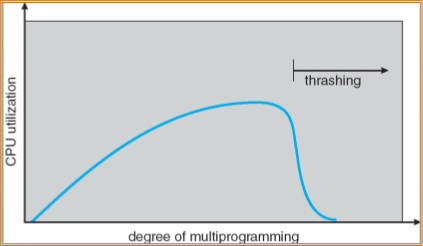
\includegraphics[scale=0.4]{images/virtual_memory/thrashing.jpg}
\caption{Thrashing}
\end{figure}

\subsection{Working-Set Model}
Defining $\Delta$ as the working-set windows (i.e.,\@ a fixed number of page references), it is possible to define ${WSS}_i$ as the working set of process $P_{i}$ (i.e.,\@ the total number of pages referenced in the most recent $\Delta$).
\begin{itemize}
\item If $\Delta$ is too small, it will not encompass entire locality;
\item If $\Delta$ is too large, it will encompass several localities;
\item If $\Delta = \infty$, it will encompass entire program.
\end{itemize}
The working-set strategy has a variable \emph{resident set}, $\overline{RT} = \dfrac{1}{T} \sum_{t=1}^T RS(t,\Delta)$.

\subsection{Page-Fault Frequency Scheme}
It is needed to establish ``acceptable'' page-fault rate ($1/c$ where $c$ is the time between two page faults). If actual rate is too low, the process loses frame. On the other hand, if actual rate is too high, process gains frame.

\paragraph{Strategy}
Run at each page fault, not at every reference. It is controlled by the time interval between page faults.
\begin{itemize}
\item If $\tau < c$, i.e.,\@ the measured page fault frequency is greater than the one acceptable, a page has to be added to the Resident Set of the process issuing this page fault;
\item If $\tau > c$, all pages not referred in that interval by the current process are eliminated from its Resident Set. The reference bit of all pages in the Resident Set are cleared.
\end{itemize}

\begin{figure}[hbtp]
\centering
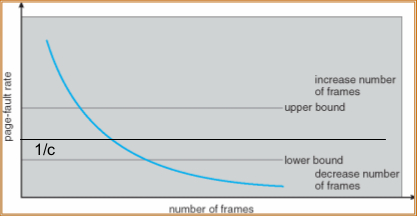
\includegraphics[scale=0.6]{images/virtual_memory/page_fault_frequency.jpg}
\caption{Page-Fault frequency scheme}
\end{figure}

\subsection{Other issues}
\paragraph{Prepaging}
To reduce the large number of page faults that occurs at process startup, prepage all or some of the pages a process will need before they are referenced but if prepaged pages are unused, I/O and memory is wasted.

Assuming $s$ pages are prepaged and $\alpha$ of the pages is used, it is needed to compare the cost of $s \cdot \alpha$ save pages faults with the cost of prepaging $s \cdot (1-\alpha)$ unnecessary pages.

\paragraph{Page size}
Page size selection must take into account fragmentation, table size, I/O overhead and locality.
\chapter{Device management}
\section{Booting a PC to run a kernel}
\begin{figure}[hbtp]
\centering
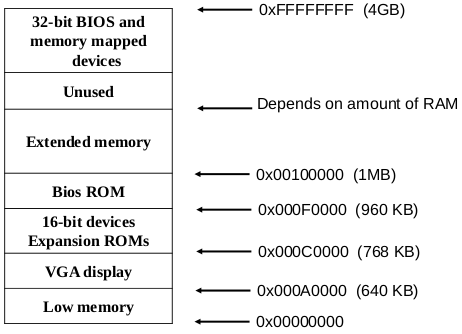
\includegraphics[scale=0.4]{images/device_management/booting_memory.png}
\caption{UNIX Memory Organization}
\end{figure}

The first PCs, which were based on the 16-bit Intel 8088 processor, were only capable of addressing 1MB of physical memory. The physical address space of an eary PC would therefore start at 0x00000000 but end at 0x000FFFFF instead of 0xFFFFFFFF.
\begin{itemize}
\item The 640KB area marked ``Low Memory'' was the \textit{only} random-access memory (RAM) that an early PC could use;
\item The 348KB area from 0x000A0000 through 0x000FFFFF was reserved by the hardware for special uses such as video display buffers and firmware held in nonvolatile memory;
\item The most important part of this reserved area is the Basic Input/Output System (BIOS), which occupies the 64KB region from 0x000F0000 through 0x000FFFFF.
\end{itemize}

Intel 80286 and 80836 processors supported 16MB and 4GB physical address spaces respectively, but the PC architects preserved the original layout for the low 1MB of physical address space for backward compatibility with existing software. Modern PCs therefore have a ``hole'' in physical memory from 0x000A0000 to 0x00100000, dividing RAM into ``low'' or \emph{conventional memory} (the first 640KB) and \emph{extended memory} (everything else).
More BIOS is located at the high end of the 32-bit address range for use by 32-bit PCI devices.

\subsection{The BIOS}
The BIOS is responsible for performing \emph{Power-On-Self-Test} and basic system initialization such as activating the video card and checking the amount of memory installed. After performing this initialization, the BIOS loads the operating system from some appropriate location such as floppy disk, hard disk, CD-ROM, or the network, and passes control of the machine to the operating system.

486 and later processors start executing at physical address 0xFFFFFFF0, which is at the very top of memory space, in an area reserved for the ROM BIOS. The first instruction is \texttt{jmp far F000:E05B} which jumps to the normal BIOS, located in the 64KB region from 0xF0000 to 0xFFFFF mentioned above. The CPU starts in \emph{real mode}, so the \texttt{jmp far} instruction is a real mode jump that restores us to low memory. In real mode, the segmented address \texttt{segment:address} translates to the physical address \texttt{segment*16 + offset}. Thus, F000:E05B translates to 0x000FE05B.

In real mode, nether Global Descriptor Table (GDT) nor Local Descriptor Table (LDT) (which, in protected mode, contain global and local segment descriptions respectively) are needed by the CPU. The code that initializes these data structures must run in real mode. When the BIOS run, it initializes the PCI bus and all the important devices it knows about (in particular VGA display), then it searches for a bootable device such as a floppy disk, hard drive or CD-ROM and when it find it, it reads the boot loader from the disk and transfers control to it.

\subsection{The Boot Loader}
The \emph{Boot Loader} is the program run by the BIOS to load the image of a kernel into RAM. Floppy and hard disks are by historical convention divided up into 512 byte regions called \emph{sectors}. If the disk is bootable, the first sector is called the \emph{boot sector}, since this is where the Boot Loader code resides. When the BIOS find a bootable floppy or hard disk, it loads the 512-byte boot sector into lowe memory, at physical address 0x7C00 through 0x7DFF and then it uses a \texttt{jmp} instruction to set the \texttt{CS:IP} to 0000:7C00, passing control to the Boot Loader.

Boot Loader important files are:
\begin{itemize}
\item \texttt{boot.s} - First, the boot loader switches the processor from real mode to 32-bit protected mode, because  it is only in this mode that software can access all the memory above 1MB in the processor's physical address space;
\item \texttt{main.c} - Second, the boot loader reads the kernel from the hard disk by directly accessing the IDE disk device registers via the x86's special I/O instructions;
\item \texttt{boot.asm} - This file is a disassembly of the boot loader. It easy to see exactly where in the physical memory all of the boot loader's code resides.
\end{itemize}

The boot loader's link and load addresses match perfectly. There is a rather large disparity between the kernel's link and load addresses. Operating system kernels often like to be linked and run at very high virtual address, such as 0xF0100000, in order to leave the lower part of the processor's virtual address space for user programs to use. Actually, it is not possible to load the kernel at \textit{physical address} 0xF0100000, then it is needed to use the processor's memory management hardware to map virtual address 0xF0100000 - link address where the kernel code \emph{expects} to run - to physical address 0x00100000 - where the boot loader \textit{actually} loaded the kernel. The kernel's virtual memory address is high enough to leave plenty of address space for user processes, it will be loaded in physical memory at the 1MB point in the PC's RAM, just above the BIOS ROM.

\section{I/O subsystem}
\begin{figure}[hbtp]
\centering
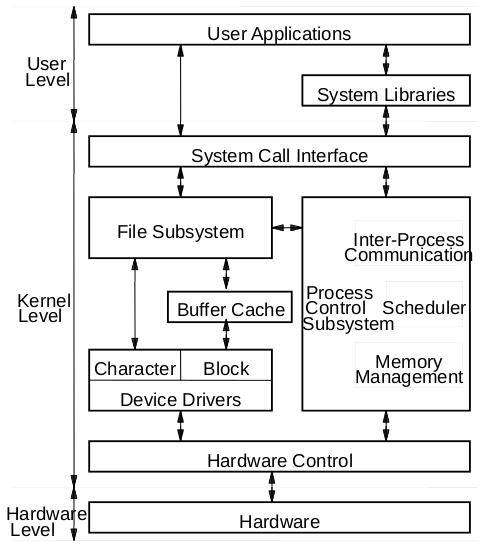
\includegraphics[scale=0.4]{images/device_management/unix_io_subsystem.png}
\caption{UNIX I/O subsystem}
\end{figure}
User application access to a wide variety of different devices is accomplished through layering and through encapsulating all the device-specific code into device drivers, while application layers are presented with a common interface for all (or at least large general categories of) devices. Most devices can be characterized as either block I/O, character I/O, memory mapped file access or network sockets. A few devices are special, such as time-of-day clock and the system timer. Most operating systems also have an escape, or back door, which allows applications to sens command directly to device drivers if needed. In UNIX this is \texttt{ioctl()} system call. \texttt{ioctl()} takes three arguments: the file descriptor for the device driver being accessed, an integer indicating the desired function to be performed and an address used for communicating or transferring additional information.

\subsection{Block and Character Devices}
Block devices are accessed one block at a time, and are indicated by a \texttt{b} as the first character in a long listing on UNIX systems. Operations supported include \texttt{read}, \texttt{write} and \texttt{seek}. Accessing blocks on a hard drive directly, without going through the filesystem structure, is called \emph{raw I/O} and can speed up certain operation by bypassing the buffering and locking normally introduced by the OS, i.e.\@ it becomes the application's responsibility to manage those issues. A new alternative is \emph{direct I/O}, which uses the normal filesystem access, but which disables buffering and locking operations. Memory mapped file I/O can be layered on top of block-device drivers. Rather than reading the entire file, it is mapped to a range of memory addresses and then paged into memory as needed using the virtual memory mechanism. Access to the file is then accomplished through normal memory access, i.e.\@ pointers, rather than through \texttt{read} and \texttt{write} system calls. This approach is commonly used for executable program code.

\begin{figure}[hbtp]
\centering
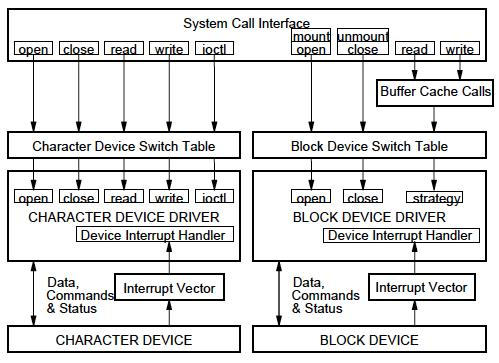
\includegraphics[scale=0.4]{images/device_management/unix_sw_interface.jpg}
\caption{UNIX software interface}
\end{figure}

Character devices are accessed one byte at a time, and are indicated by a \texttt{c} in UNIX systems. Supported operations include \texttt{get} and \texttt{put}, with more advanced functionality such as reading an entire line supported by higher-level library routines.

\subsection{Filesystem data structures}
In the original UNIX filesystem, the physical disks is divided into logical disks called \emph{partitions}. Each partition is a standalone filesystem. Each device in the system is characterized by its own major device number and each partition has an associated minor device number which the device drivers uses to access the raw filesystem. The major/minor device number combination is used as an handle into device switch table. In particular, the major number acts as an index, and the minor number is passed as an argument to the driver routines so that they can recognize the specific instance of a device.

Each filesystem contains:
\begin{itemize}
\item a \emph{boot block} located in the first few sectors of a filesystem. The boot block contains the initial bootstrap program used to load the operating system. Typically, the first sector contains a bootstrap program that reads in a larger bootstrap program from the next few sector, and so forth;
\item a \emph{superblock} describes the state of the filesystem: the total size of the partition, the block size, pointers to a list of free blocks, the i-node number of the root directory, magic number, etc.;
\item a linear \emph{array of i-nodes}. There is a one to one mapping of files to i-nodes and viceversa. An i-node is identified by its \emph{i-node number}, which  contains the information needed to find the i-node itself on the disk. Thus, while users think of files in terms of file names, UNIX thinks of files in terms of i-nodes.
\item a \emph{data blocks} containing the actual content of files.
\end{itemize}

System calls like \texttt{mkfs} can be used to create (format) the filesystem (partition). Indeed, it creates the superblock, the i-node list, the list of free blocks and the root node for the new filesystem. Other system calls like \texttt{fsck}, instead, are used to check and repair the filesystem.

Therefore, it is simple to understand that there is a similarity between normal files and device in a UNIX filesystem: both are characterized by an i-node.

\begin{figure}[hbtp]
\centering
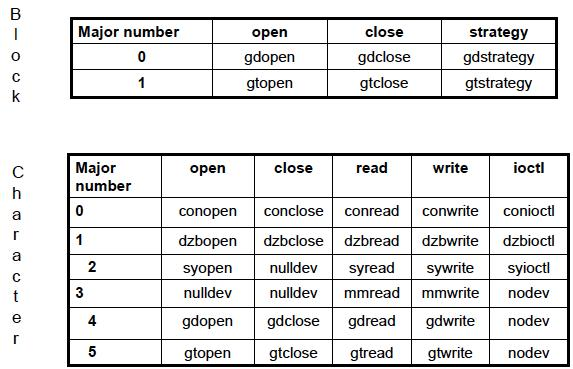
\includegraphics[scale=0.4]{images/device_management/unix_switch_tables.jpg}
\caption{UNIX switch tables}
\end{figure}

\paragraph{Open system call for I/O devices}
\begin{enumerate}
\item Convert pathname into i-node;
\item Increase the i-node reference counter;
\item Allocate an element into user file table and system file table;
\item Get major and minor number from i-node;
\item Save content using \texttt{setjmp}\footnote{Saves the current context (environment) in the stack. Used to backtrack in case of errors, instead of a chain of \texttt{return} statements} to resolve a possible \texttt{longjmp} executed by the driver;
\item If device is a block device:
\begin{enumerate}
\item Use major number as an index into block device switching table;
\item Call open procedure of the driver associated to the index above passing minor number and mode;
\end{enumerate}
\item Otherwise:
\begin{enumerate}
\item Use major number as an index into character device switching table;
\item Call open procedure of the driver associated to the index above passing minor number and mode;
\end{enumerate}
\item If open fails, decrease counters in file and i-node tables.
\end{enumerate}

\subsection{Terminal driver}
A multiplicity of I/O devices are regarded as ``terminals'' in Unix systems. A terminal is a character-oriented device, comprising streams of characters received from and sent to the device. Although characters streams are structured, incorporating control characters, escape codes and special characters, the I/O protocol is not structured as would be the I/O protocol of smart terminals. Terminals provide job control facilities: interactively, the user and the terminal can send control characters that suspend the current running job, reverting to the interactive job control shell that spawned the job and can run commands which place jobs in background or which switch a background job into foreground, without suspending it if necessary.

In UNIX, a terminal device comprises the underlying \emph{device driver}, responsible for the physical control of the device hardaware via the I/O instructions and handling device interrupt requests, and the \emph{line discipline}, as shown in figure~\ref{unix_line_discipline}. A line discipline is independent from the actual device hardware, and the same line discipline can be used for a terminal concentrator device responsible for multiple controlling terminals as for a pseudoterminal. Line disciplines can be setup by functions or system calls. They are the same across all terminal devices and independent from the actual hardware, dealing as they do in the simple abstractions provided by device drivers: transmit and receive a character and set different hardware states. Each terminal device can be switched among multiple line disciplines.

\begin{figure}[hbtp]
\centering
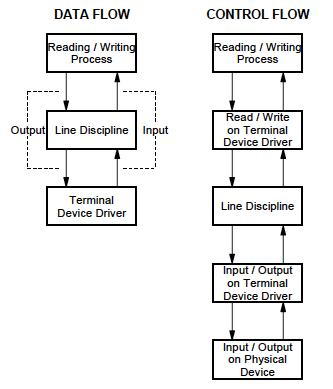
\includegraphics[scale=0.6]{images/device_management/unix_line_discipline.jpg}
\caption{UNIX line discipline}
\label{unix_line_discipline}
\end{figure}

Every line discipline may operate in two modes:
\begin{itemize}
\item \textbf{Raw mode}: the line discipline transfers data between a terminal and a process without any conversion. The \texttt{enter} character has no specific meaning in this mode. The behavior of the raw mode can be set using the \texttt{ioctl} system call;
\item \textbf{Canonical mode}: characters are got into kernel buffer and passed to the process only when \texttt{ENTER} is pressed. The user input is converted for the receiving process and the process output is converted for the user. It manages \texttt{backspace}, formatting characters such as \texttt{tab} and \texttt{enter} and special characters such as \texttt{Ctrl-C}, \texttt{Del} and \texttt{Ctrl-D}.
\end{itemize}

The POSIX standard replaces the \texttt{ioctl} system call entirely, with a set of library functions with standardized names and parameters. The POSIX \texttt{termio} data structure is the data structure used by all of the terminal library calls.
\begin{verbatim}
struct termios {
  tcflag_t c_iflag;  // Input mdoes
  tcflag_t c_oflag;  // Output modes
  tcflag_t c_cflag;  // Control modes
  tcflag_t c_lflag;  // Local modes
  cc_t c_cc[NCCS];   // Control characters
};
\end{verbatim}
Each process in the system has either a single controlling terminal, or no controlling terminal at all. A process inherits its controlling terminal from its parent, and the only operations upon a process are acquiring a controlling terminal, by a process that has no controlling terminal, and relinquishing it, by a process that has a controlling terminal. The standard defines the \texttt{O\_NOCTTY} flag for the \texttt{open} system call. A process with no controlling terminal opens a terminal device file that is not already the controlling terminal for some other process, without specifying the \texttt{O\_NOCTTY} flag.

\subsubsection{\texttt{getty}}
\texttt{getty} (get teletype) is a typical UNIX system program used to manage physical and virtual terminals. When it detects a connection, it prompts for a username password an runs the ``login'' program to authenticate the user.

At the login phase, the \texttt{init} process reads \texttt{/etc/inittab} and executes a \texttt{getty} process for each known terminal that has been switched on. Then, \texttt{getty} calls the system call \texttt{open} related to the terminal, which makes the process wait for the hardware connection has been established. The \texttt{getty} program, through system call \emph{exec}, becomes the \texttt{login} process, which runs, exploiting system call \texttt{exec}, the user selected shell reading the last field of the username record in file \texttt{/etc/passwd}.

\subsection{Buffer cache}
In order to speedup the read request from a device, it is possible to use buffers and/or caches which allow a faster communication to take place

When the kernel is asked to serve a \textbf{read} request from disk, it tries to read the data from the \emph{buffer cache}. If the data are in the cache, the data are returned to the user process without any disk access, otherwise the kernel reads a block of data from disk and stores it in the buffer cache, trying to keep it in memory as long as possible, for a possible future usage.

When the kernel is asked to serve \textbf{write} request to disk, it puts the data in the buffer cache. In this way, data stay in memory for possible read operations and any change of the data is performed in memory rather than on disk.

The buffer cache management tries to minimize the number of disk accesses by \emph{reading ahead} the data that have high probability\footnote{According to the space and temporal locality principle} to be referenced in the near future and by delaying as much as possible the transfer of the content of the buffer cache to disk (\emph{delayed write}).

\subsection*{Read system call}
\begin{verbatim}
procedure read
input:  user file descriptor
        user buffer address
        number of bytes to read
output: number of bytes copied in the user buffer
{
  while(! complete number of bytes to read) {
    convert offset to byte in a block (using bmap);
    compute the offset within a block
      and the number of byte to read;
    if(number of byte to read == 0)
      break;  /* tries to read beyond the end of file */
    read a block (using bread or breada);
    copy data from kernel buffer to user space;
    release buffer (using brelse);
    
    return number of bytes; 
}
\end{verbatim}

\subsection*{Block read: \texttt{bread}}
\begin{verbatim}
procedure bread
input:  filesystem block number (blockno)
output: buffer containing requested block
{
  buffer = getblock(block blockno);
  if(data in buffer are valid)
    return buffer;
  start disk I/O read for block blockno into buffer;
  sleep(event: disk I/O read completed);
  return buffer;
}
\end{verbatim}

\subsection*{Acquiring a block: \texttt{getblk}}
\begin{verbatim}
procedure getblk
input:  device number
output: locked buffer to be used for storing the block
{
  while(buffer not found) {
    if(block is present in its hash queue) {
      /* Case 5 */
      if(buffer is locked) {
        sleep(event: buffer unlocked);
        continue;
      }
      /* Case 1 */
      mark buffer 'locked';
      remove buffer from free list;
      return buffer;
    } else {
      if(free list is empty) {
        /* Case 4 */
        sleep(event: freed buffer);
        continue;
      }
      remove buffer from free list;
      if(buffer marked 'delayed write') {
        /* Case 3 */
        asynchronous disk write of buffer;
        continue;
      }
      /* Case 2 */
      remove buffer from old hash queue;
      put buffer into new hash queue;
      return buffer;
    }
  }
}
\end{verbatim}

\subsection*{Block release: \texttt{brelse}}
\begin{verbatim}
procedure brelse
input:  locked buffer
output: none
{
  wake up all processes waiting for any free buffer;
  wake up all processes waiting for this buffer;
  disable interrupts;
  if(buffer contents are valid and buffer not old) {
    put buffer in free list queue;
  else
    put buffer in free list head;
  enable interrupts;
  mark buffer unlocked;
}
\end{verbatim}

\subsection*{Block write: \texttt{bwrite}}
\begin{verbatim}
procedure bwrite
input:  buffer to write
output: none
{
  start disk I/O write of buffer;
  if(synchronous I/O) {
    sleep(event: disk I/O write completed);
    brelse(buffer);
  } else if(buffer is marked delayed write)
    mark buffer 'old';
}
\end{verbatim}

\subsection*{Block read ahead: \texttt{breada}}
\begin{verbatim}
procedure breada
input:  filesystem block number for immediate read (blkno1)
        filesystem block number for asynchronous read (blockno2)
output: buffer containing data from immediate read (buffer1)
{
  if(buffer with blkno1 not present in buffer cache) {
    buffer1 = getblk(block blkno1);
    if(data in buffer1 are not valid)
      start disk I/O read for blockno1 into buffer1;
  }
  if(buffer with blkno2 not present in buffer cache) {
    buffer2 = getblk(block blkno2);
    if(data in buffer2 are valid)
      brelse(buffer2);
    else
      start disk I/O read for block blkno2 into buffer2;
  }
  if(buffer with blkno1 present in buffer cache) {
    buffer1 = bread(blkno1);
    return buffer1;
  }
  sleep(event: blkno1 disk I/O read completed);
  return buffer1;
}
\end{verbatim}

\chapter{File system}
The \emph{file system} is a layer of OS which transforms block interface of disks (or other block devices) into files, directories, etc.
A \emph{file} is an abstract data type that associates the name to its data. Data are normally referred as record but they are organized in blocks. There is no correspondence between blocks and records. Blocks are not accessed directly, because in between there are strategies on how accessing the block which may optimize the block access.

\section{Overview}
File systems have traditionally divided the disk into equally sized blocks to simplify their design and limit the worst-case fragmentation. When files are allocated, only whole blocks can be allocated to individual files. But, as file sizes are often not multiples of the file system block size, this design inherently results in the last blocks of files  occupying only a part of the block, resulting in what is called \emph{internal fragmentation}. This waste of space can be significant if the file system stores many small files and can become critical when attempting to use higher block sizes to improve performance.

\begin{figure}[hbtp]
\centering
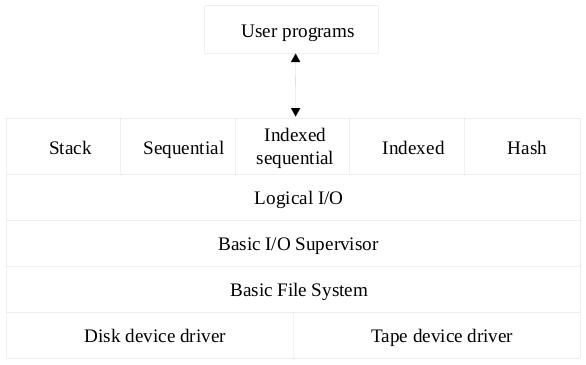
\includegraphics[scale=0.4]{images/file_system/logical_level_file_access.png}
\caption{Logical levels for file access}
\end{figure}

\subsection{Regular file}
Data in a file are reachable using common operations such as creation, writing, reading, deleting, etc.

Different OSs keep track of different file attributes, including:
\begin{itemize}
\item File type;
\item File system type;
\item Volume;
\item Starting address;
\item Size;
\item Owner;
\item Access rights;
\item Use information (when/who has last written/read/modified the file or its attributes).
\end{itemize}
Files are organized in directories and subdirectories.

\subsection{Disk file organization}
There are three major methods to store files on disks: contiguous, linked and indexed.

\subsubsection{Contiguous allocation}
Contiguous allocation requires that all blocks of a file are kept together one after the other. In this way, access is very fast because reading consecutive blocks requires no movement of the disk heads or one small step to the next adjacent cylinder.

\begin{figure}[hbtp]
\centering
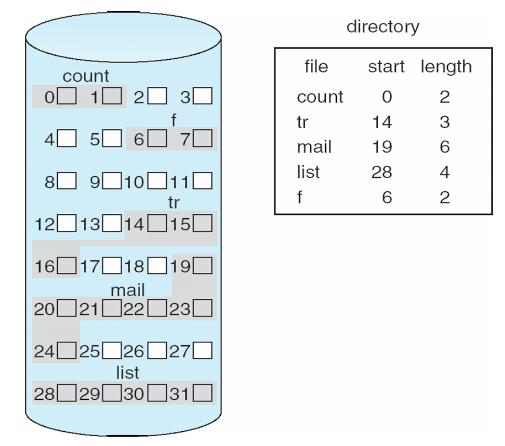
\includegraphics[scale=0.35]{images/file_system/contiguous_allocation.png}
\caption{Contiguous allocation}
\end{figure}

This type of allocation has the same issues of the contiguous allocation in main memory (e.g.\@ first fit, best fit, fragmentation problems). Problems can arise when files grow, or if the exact file size is unknown at creation time. In fact, an over-estimation will cause external fragmentation and space waste, while under-estimation may cause the relocation of the file.

\subsubsection{Linked allocation}
Disk files can be stored as linked lists, with the expense of the storage space consumed by each link (i.e.\@ for each block, 4 bytes are lost to store the address of next block). Linked allocation has no external fragmentation, does not require to know a priori the file size and, therefore, allows files to grow dynamically. This allocation permits only sequential access to files because it is needed to traverse the entire series of blocks and it is dangerous because administration data (link) together with user data and it has the disadvantage that, if a pointer is lost or damaged, the entire file is unreachable and corrupted.

\begin{figure}[hbtp]
\centering
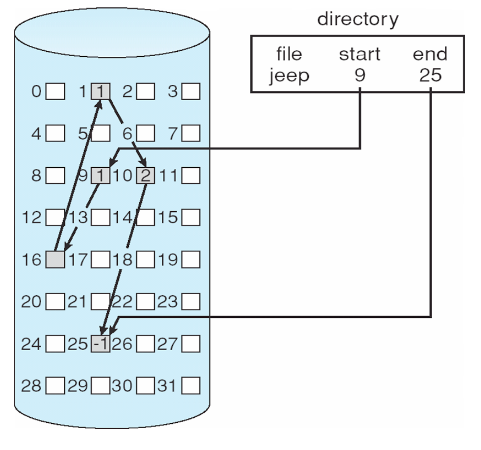
\includegraphics[scale=0.35]{images/file_system/linked_allocation.png}
\caption{Linked allocation}
\end{figure}

The \textbf{File Allocation Table (FAT)}, adopted by \emph{DOS file system}, is an improvement to basic linked allocation. The main idea is to separate administration data from user data adopted. Directories are associated with a number representing both the pointer to the first block of data and an index into FAT. Each entry of the FAT contains the index of next block, providing separation between administration and user data and immediate access to the first block. Therefore, small files (which are the most common) can be immediately referenced.

\begin{figure}[hbtp]
\centering
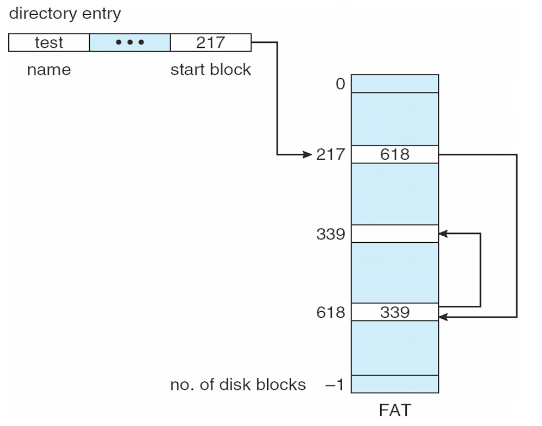
\includegraphics[scale=0.35]{images/file_system/fat.png}
\caption{File Allocation Table (FAT)}
\end{figure}

\subsubsection{Indexed allocation}
Indexed allocation keeps all the indexes into a single block (i.e. block of indexes) for each file instead of spreading them all over the file system or storing them in a FAT. When a file is opened, its index block is opened too and it is possible to access the its blocks wherever they are. Some disk space is wasted because an entire index block must be allocated for each files. There are several approaches to implement the index block:
\begin{itemize}
\item Linked Scheme: An index block is one disk block, which can be read and written in a single disk operation. The first index block contains some header information, the first N block addresses, and if necessary a pointer to additional linked index blocks;
\item Multi-Level Index: The first index block contains a set of pointers to secondary index blocks, which in turn contain pointers to the actual data blocks.
\end{itemize}

\begin{figure}[hbtp]
\centering
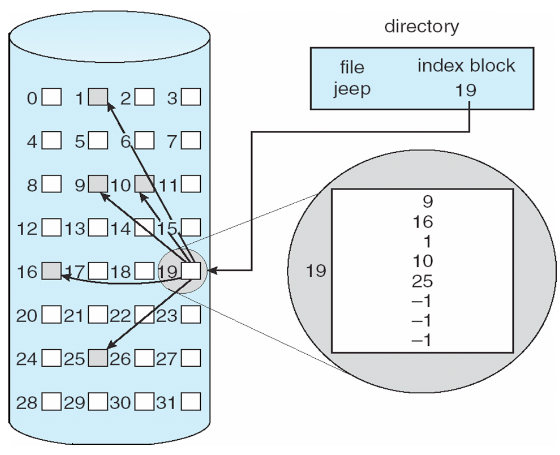
\includegraphics[scale=0.35]{images/file_system/indexed_allocation.png}
\caption{Indexed allocation}
\end{figure}

\section{UNIX file system organization}
UNIX adopts a \emph{combined scheme} in its inodes. In fact, it stores 10 data block pointers directly in the inode, and then singly, doubly and triply indirect pointers provide access to more data blocks as needed.

\begin{center}
\begin{tabular}{|c|c|c|c|}
\hline 
Boot block & Superblock & Inode list & Data blocks \\ 
\hline 
\end{tabular} 
\end{center}

\begin{itemize}
\item The first block is the \emph{boot block} containing the bootstrap code loaded and executed at system power on.
\item The \emph{superblock} describes the file system state, i.e.\@ size, number of files included, free list of inodes and data blocks, etc.
\end{itemize}

\paragraph{Inode} The \emph{inode} contains information about the owner, file type (regular, directory, special, \dots), access rights, access times, link number, file size and table of the data block addresses on disk. Those information can be retrieved exploiting command \texttt{ls -l}.

\begin{figure}[hbtp]
\centering
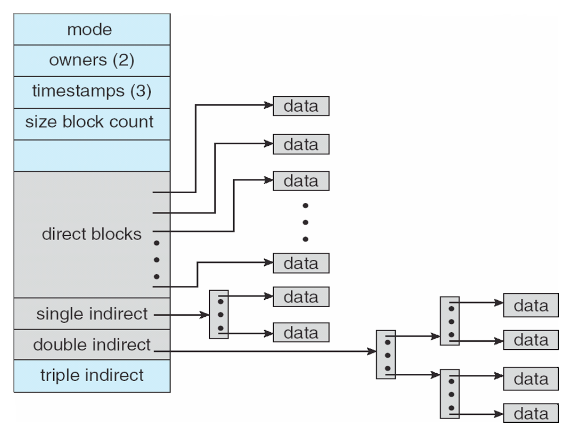
\includegraphics[scale=0.35]{images/file_system/unix_combined_scheme.png}
\caption{The UNIX allocation of disk space}
\end{figure}

\subsection{Functions for file system management}
Table~\ref{system_mgmt_upper_layers} includes functions directly used by system calls, which exploit functionality provided by procedures contained in table~\ref{system_mgmt_lower_layers}. Here, the functions placed at the lower layer, are used directly by the buffer cache, e.g.\@ get block, block release, block read. The most used is \texttt{getblk} used to retrieve a block at any access. Those functions are exploited by some allocation algorithms, placed on top of them, e.g.\@ copy, delayed write.

\begin{table}
\centering
\begin{tabular}{|c|c|c|cc|cc|}
\hline 
\multicolumn{3}{|c|}{\texttt{namei}} & \multirow{2}{*}{\texttt{alloc}} & \multirow{2}{*}{\texttt{free}} & \multirow{2}{*}{\texttt{ialloc}} & \multirow{2}{*}{\texttt{ifree}} \\\cline{1-3} 
\texttt{iget} & \texttt{iput} & \texttt{bmap} & & & & \\ 
\hline 
\end{tabular}
\caption{Upper layers}
\label{system_mgmt_upper_layers}
\end{table} 

\begin{table}
\centering
\begin{tabular}{|c|c|c|c|c|}
\hline 
\multicolumn{5}{|c|}{buffer allocation algorithm} \\ 
\hline 
\texttt{getblk} & \texttt{brelse} & \texttt{bread} & \texttt{breada} & \texttt{bwrite} \\ 
\hline 
\end{tabular} 
\caption{Lower layers}
\label{system_mgmt_lower_layers}
\end{table}

\paragraph{\texttt{iget}} It is called by system call \texttt{open}. It locks the inode, allocates in memory a copy of the inode describing a file and returns an unlocked inode with reference count incremented by one. If the inode free list is empty, the kernel returns an error.

\paragraph{\texttt{iput}} It is called by system call \texttt{close}. It locks the inode and decrements the reference count by one. If the reference count is 0, the inode is written on disk if modified and its copy is released from the inode free list. If the link~count \footnote{Number of names referring to that object.} is 0, the kernel releases all the data blocks of the file and its disk inode.

Reference counter and link counter may differ, for example, if a file is created (system call \texttt{creat}) and immediately unlinked the reference counter is one while the link counter is zero. In this case, only the process creating the file has the possibility to access the file because it knows its file descriptor, thus it may use the file as a temporary one. When the process closes (system call \texttt{close}) the file, both reference and link counters are zero and, therefore, the kernel can remove the file.

\paragraph{\texttt{bmap}} It converts the file offset in the corresponding physical block on disk. Given the offset, it uses the inode pointers to identify disk block where the information is stored and returns a pointer to the disk block.

\paragraph{\texttt{namei}} It returns the inode of a file, given its pathname. It analyzes a pathname component at a time and finds the corresponding inode. The pointer to the inode of the process working directory is stored in the user area \footnote{Common kernel memory area to all process. Kernel uses this are to store the parameters of the currently running process}. It implements a non trivial and expensive operation. In fact it is used only once when a file is opened, then the file descriptor is used to reach the file.

\paragraph{\texttt{ialloc}} It is called by system call \texttt{open} with \texttt{O\_CREAT} flag. It assigns a disk inode to a file that has to be created.

\paragraph{\texttt{ifree}} It is called by system call \texttt{unlink}. It releases the inode of a file that has been remove, and is not currently in use, i.e.\@ reference count greater than zero.

\paragraph{\texttt{alloc}} It is called when the file is written and a new data block is needed. It allocates the first free block number in the superblock free list. If this block is the last block available in the superblock's list, it contains all the addresses to free blocks in the disk. Thus, the operating system will use the number of the block as pointer to a block storing the next element of the linked list, which is integrally loaded into the cache and the previous block, now empty, can be allocated for the process which made the request for it.

\paragraph{\texttt{free}} It provides the same functionalities of the \texttt{ifree} routine saw previously.

\subsection{File system system calls}
\begin{itemize}
\item Return a descriptor: \texttt{open}, \texttt{creat}, \texttt{dup}, \texttt{pipe}, \texttt{close};
\item Use \texttt{namei}: \texttt{open}, \texttt{creat}, \texttt{chdir}, \texttt{chroot}, \texttt{chown}, \texttt{chmod}, \texttt{stat}, \texttt{link}, \texttt{unlink}, \texttt{mknod}, \texttt{mount}, \texttt{umount};
\item Allocate inode: \texttt{creat}, \texttt{mknod}, \texttt{unlink};
\item Attributes: \texttt{chown}, \texttt{chmod}, \texttt{stat};
\item I/O: \texttt{read}, \texttt{write}, \texttt{seek};
\item File system structure management: \texttt{mount}, \texttt{umount}, \texttt{chdir}, \texttt{chroot}.
\end{itemize}

\paragraph{open} \texttt{int fd = open(char* pathname, int flags, mode\_t mode);}

It returns a \emph{file descriptor} associated to \texttt{pathname}. The parameter \texttt{flags} must include one of the access modes: \texttt{O\_RDONLY}, \texttt{O\_WRONLY} or \texttt{O\_RDWR} standing for read-only, write-only or read write, respectively. In addition, zero or more file creation flags and file status flags can be bitwise-or'd in \texttt{flags}, e.g.\@ create file if not existing, truncate it, append the content, no writing delay, exclusive access.

\begin{figure}[hbtp]
\centering
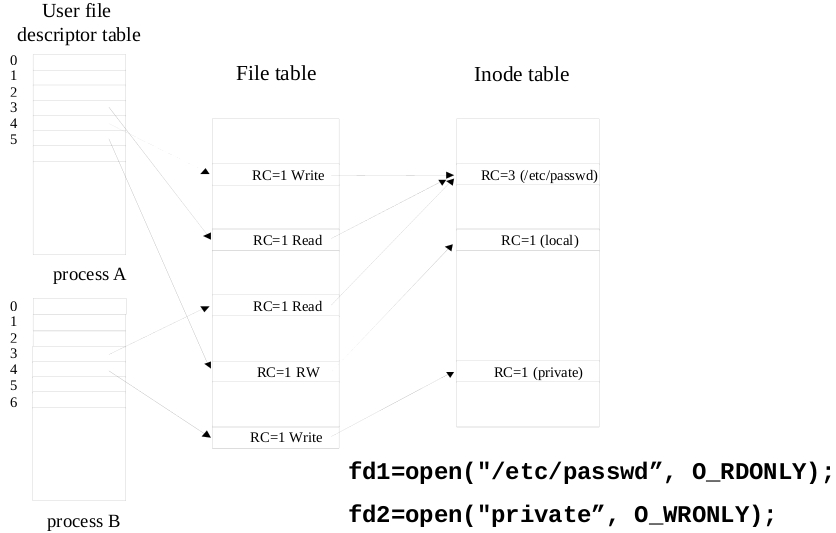
\includegraphics[scale=0.4]{images/file_system/open_system_call.jpg}
\caption{UNIX open system call}
\end{figure}

\paragraph{read} \texttt{ssize\_t number = read(int fd, void* buffer, size\_t count);}

It attempts to read up to \texttt{count} bytes from file descriptor \texttt{fd} into the buffer starting at \texttt{buf}. When the functions completes with success, it returns the number of bytes read, and the file position is advanced by this number. The while \texttt{count} cycle ends:
\begin{itemize}
\item because \texttt{count} is satisfied;
\item because of \emph{EOF}, different than reading a block with zero pointer in its node;
\item because of read error from the device;
\item because of error during the copy to the user buffer.
\end{itemize}
The I/O parameters are copied in the user area:
\begin{itemize}
\item \emph{mode}: read or write;
\item \emph{count}: number of bytes to be read or written;
\item \emph{offset}: where to begin the I/O operation;
\item \emph{address}: source or destination;
\item \emph{flag}: kernel or user space;
\item flag directory;
\item possible changed root.
\end{itemize}
If more than one process have to access the same file and one of them wants to access it in write mode, file and record locking have to be used to guarantee the mutual exclusion access.

\subparagraph{Read ahead}
While a process executes the system call \texttt{read} of two logical sequential blocks, the kernel assumes that all its successive calls will be sequential. At every iteration of the reading cycle, the kernel stores the next logical block number in the inode in memory and, in the next iteration, it tests if the current block number is equal to the saved one. If they are equal, the kernel computes the physical block number for the read ahead using \texttt{bmap} routine and stores its value in the user area so that it can be used by \texttt{breada}.

\paragraph{write}
\texttt{ssize\_t write(int fd, const void *buf, size\_t count);}

It writes up to \texttt{count} bytes to the file referenced by the file descriptor \texttt{fd} from the buffer starting at \texttt{buf}. On success, the number of bytes written are returned (zero indicates nothing was written). On error, -1 is returned.

If the write offset does not correspond to an already allocated block, the kernel allocates a new block and updates the pointer structure, possibly allocating one or more indirect blocks. If, instead, the kernel has to write only part of a block, it must read the block from disk. Delayed write is particularly suited to pipes and temporary files.

\paragraph{lseek}
\texttt{off\_t lseek(int fd, off\_t offset, int whence);}

It repositions the file offset of the open file associated with the file descriptor \texttt{fd} to the argument \texttt{offset} according to the directive \texttt{whence} as follows:
\begin{itemize}
\item \texttt{SEEK\_SET}: The file offset is set to \texttt{offset} bytes.
\item \texttt{SEEK\_CUR}: The file offset is set to its current location plus \texttt{offset} bytes.
\item \texttt{SEEK\_END}: The file offset is set to the size of the file plus \texttt{offset} bytes.
\end{itemize}
It allows the file offset to be set beyond the end of the file,but this does not change the size of the file. If data is later written at this point, subsequent reads of the data in the gap (a \emph{hole}) return null bytes until data is actually written into the gap. Upon successful completion, it returns the resulting offset location as measured in bytes from the beginning of the file.  On error, the value -1 is returned.

\paragraph{close}
\texttt{int close(int fd);}

It closes a file descriptor, so that it no longer refers to any file and may be reused. Any record locks held on the file it was associated with, and owned by the process, are removed (regardless of the file descriptor that was used to obtain the lock). If \texttt{fd} is the last file descriptor referring to the underlying open file description, the resources associated with the open file description are freed; if the file descriptor was the last reference to a file which has been removed using \texttt{unlink}, the file is deleted. It returns zero on success. On error, -1 is returned.

If the inode reference count is greater than one, it decrements the counter and return. If the inode reference count is one, the kernel releases, by means of \texttt{iput}, the inode allocated in memory by the \texttt{open} system call, the corresponding entry in the inode table and the entry in the user file description tables. When a process exits, the kernel closes all its file descriptor still open. 

\paragraph{creat}
\texttt{int creat(const char *pathname, mode\_t mode);}

It is equivalent to calling \texttt{open} with flags equal to \texttt{O\_CREAT | O\_WRONLY | O\_TRUNC}. If the file does not exist, it is create with the specified name and mode. The kernel analyzes the pathname by means of \texttt{namei} and when the last component is parsed, it allocates a free inode, it stores the name in the first free entry of the last parsed directory name and opens the file. If the file exists, parsing it pathname, the kernel finds its inode, it initializes the file dimension to 0 and releases all its data blocks.

If the process calling \texttt{creat} has the write permission, and the file exists, the file owner and the access permission do not change. The kernel does not verify that the parent directory of existing file has the write permission because the directory content does not change.

\paragraph{mknod}
\texttt{int mknod(const char *pathname, mode\_t mode, dev\_t dev);}

It creates a filesystem node (file, device special file, or named pipe) named \texttt{pathname}, with attributes specified by \texttt{mode} and \texttt{dev}. The \texttt{mode} argument specifies both the file mode to use and the type of node to be created and it should be a combination (using bitwise OR) of one of the file types listed below and zero or more of the file mode bits. The file type must be one of \texttt{S\_IFREG}, \texttt{S\_IFCHR}, \texttt{S\_IFBLK}, \texttt{S\_IFIFO}, or \texttt{S\_IFSOCK} to specify a regular file (which will be created empty), character special file, block special file, FIFO (named pipe), or UNIX domain socket, respectively. If the file type is \texttt{S\_IFCHR} or \texttt{S\_IFBLK}, then \texttt{dev} specifies the major and minor numbers of the newly created device special file; otherwise it is ignored. It returns zero on success, or -1 if an error occurred.

It may be used to create named pipes which are pipes remaining in the file system and permit communication among processes which are not parent and child.

\paragraph{chdir}
\texttt{int chdir(const char *pathname);}

It shall cause the directory named by the pathname pointed to by the \texttt{pathname} argument to become the current working directory; the starting point for \texttt{pathname} searches for pathnames not beginning with \texttt{/}. Upon successful completion, 0 shall be returned. Otherwise, -1 shall be returned and the current working directory shall remain unchanged. 

The kernel decrements the reference count, releases the old directory inode and stores the inode of the new directory in the user area. The current directory inode is released after the process exits or calls again \texttt{chdir}.

\paragraph{chroot}
\texttt{int chroot(const char *pathname);}

It changes the root directory of the calling process to that specified in \texttt{path}. This directory will be used for pathnames beginning with /. The root directory is inherited by all children of the calling process. On success, zero is returned. On error, -1 is returned. Only privileged process can call \texttt{chroot}.

The kernel keeps a global variable pointer to the root inode. This call does not change the current working directory and does not close open file descriptors.

\paragraph{chown - chmod}
These operations change the inode, not the file content. To change the file owner or permissions, the process must be owner of the file or have superuser privileges. These system calls both return zero on success and -1 on error.
\\
\texttt{int chown(const char *pathname, uid\_t owner, gid\_t group);}

It changes the owner and group of a file specified by \texttt{pathname}.
\\
\texttt{int chmod(const char *pathname, mode\_t mode);}

It changes the permissions of a file specified by \texttt{pathname}.

\paragraph{stat - fstat} These functions return information about a file. No permissions are required on the file itself. These system calls both return zero on success and -1 on error.
\\
\texttt{int stat(const char *pathname, struct stat *buf);}

It stats the file pointed to by \texttt{pathname} and fills in \texttt{buf}.
\\
\texttt{int fstat(int fd, struct stat *buf);}

It is identical to \texttt{stat}, except that the file to be stat-ed is specified by the file descriptor \texttt{fd}.

The \texttt{stat} structure is defined in \texttt{stat.h} as follows:

\begin{verbatim}
struct stat {
  dev_t     st_dev;     /* ID of device containing file */
  ino_t     st_ino;     /* inode number */
  mode_t    st_mode;    /* protection */
  nlink_t   st_nlink;   /* number of hard links */
  uid_t     st_uid;     /* user ID of owner */
  gid_t     st_gid;     /* group ID of owner */
  dev_t     st_rdev;    /* device ID (if special file) */
  off_t     st_size;    /* total size, in bytes */
  blksize_t st_blksize; /* blocksize for file system I/O */
  blkcnt_t  st_blocks;  /* number of 512B blocks allocated */
  time_t    st_atime;   /* time of last access */
  time_t    st_mtime;   /* time of last modification */
  time_t    st_ctime;   /* time of last status change */
};
\end{verbatim}

\end{document}